\documentclass[10.5pt]{report}
\usepackage[a4paper,margin=0.9in]{geometry}
\usepackage{amsmath,amssymb}
\usepackage{booktabs}
\usepackage{longtable}
\usepackage{graphicx}
\usepackage[colorlinks=true,linkcolor=blue,citecolor=blue,urlcolor=blue]{hyperref}
\usepackage{xcolor}
\usepackage{titlesec}
\usepackage{caption}
\usepackage{enumitem}
\usepackage{array}
\usepackage{microtype}
\definecolor{hbblue}{HTML}{2A4D8F}
\titleformat{\chapter}[display]{\bfseries\Large\color{hbblue}}{\chaptertitlename\ \thechapter}{6pt}{\Large}
\titleformat{\section}{\bfseries\large\color{hbblue}}{\thesection}{6pt}{}
\captionsetup{font=small,labelfont=bf}
\setlist[itemize]{topsep=2pt,itemsep=2pt}
\setlist[enumerate]{topsep=2pt,itemsep=2pt}

\newcommand{\um}{\,\mu\text{m}}
\newcommand{\mm}{\,\text{mm}}

\title{\textbf{\LARGE Aperture Optimization for Pinhole Sunglasses}\\[0.25cm]
\textcolor{hbblue}{\Large A Complete Theoretical and Computational Study}\\[0.4cm]
\normalsize\itshape Wave-optics blur minimization, brightness constraints, human-vision
acuity modeling, and clinical validation --- scoped strictly to single-aperture
optimization; multi-hole array/ghosting questions are out of scope for this document.}
\author{}
\date{}

\begin{document}
\maketitle
\tableofcontents

\chapter*{Abstract}
\addcontentsline{toc}{chapter}{Abstract}

This report consolidates every theoretical model, numerical sweep, and validation
result this project has produced on a single question: \emph{for a myopic eye viewing
through a single circular pinhole aperture in an otherwise opaque film, what aperture
diameter is optimal, and by which criterion?} It deliberately excludes the project's
separate multi-hole array, ghosting, packing-geometry, and lens-material work, which
answer a different question (how to \emph{tile} many holes safely) and are documented
elsewhere.

Four largely independent modeling efforts are covered, each with its own governing
equations, numerical implementation, and full-grid sweep across 15 apertures
($75$--$2000\um$) and 8 myopia levels ($0$--$8\,$D): (1) an exact scalar
Angular-Spectrum-Method wave-optics pipeline from pinhole to retina, whose blur-only
optimum is the project's headline number; (2) a brightness-constrained variant of the
same pipeline, which shows that a minimum-illuminance floor moves the optimum by
roughly $2$--$3\times$ into the clinically-observed bracket; (3) a human-vision layer
(MTF, contrast sensitivity, Strehl ratio, Watson--Yellott pupil model, troland
photometry) built on top of the same optics, producing a predicted logMAR acuity
surface; and (4) a structurally independent ideal-observer Monte Carlo acuity model
(R7acuity), built specifically to cross-check (3) with a different architecture.

A significant fraction of this project's actual scientific content is a documented
\emph{physics audit}: a real lens-phase/retina-propagation wavelength bug was found,
independently re-derived two ways, and fixed, moving the blur-only optimum aperture by
up to $+150\%$ at some myopia levels; a separate Python import-shadowing bug meant two
previously-published acuity-validation results had silently never been evaluated
against the corrected optics at all, and both were re-run once the shadowing was
fixed. Both corrections, and their full before/after numbers, are reported here in
full --- including the honest result that neither acuity model achieves statistical
significance against the two available clinical datasets (Wang 2009, $n=5$; Kim et al.
2017, one aggregate point), a negative result this report does not soften.

The synthesis chapters bring these efforts together: an aperture-optimum comparison
across four different blur-percentile definitions ($r_{EE}50\%/70\%/80\%/90\%$),
including a previously-undocumented numerical saturation artifact at low myopia that
is identified and quantified rather than silently averaged over; a full corrected-vs-deprecated
optics comparison; and a cross-model summary table spanning every method in this
report. No single "recommended aperture" is asserted anywhere in this document --- each
chapter reports what its own model predicts, under its own stated assumptions, and the
final synthesis chapter shows how those predictions relate to one another and to the
two independently-documented patents in this space, without collapsing them into one
number.

\chapter{Introduction and Scope}
\label{ch:introduction}

\section{The problem}

Pinhole glasses are a well-known, non-refractive way to improve a myopic
(short-sighted) eye's perceived sharpness: restricting the eye's entrance aperture
increases depth of focus, so a blurred retinal image sharpens even though the eye's
own optical power is unchanged. The IYPT-style problem statement motivating this
project's whole body of work is: \emph{investigate the optimal arrangement of pinholes
in an opaque film to produce sunglasses that reduce light intensity and help correct
short-sightedness.} That statement bundles two physically distinct design questions:

\begin{enumerate}
\item \textbf{Aperture size} --- for a single hole, what diameter minimizes retinal
  blur for a myopic eye, and how does a brightness (light-transmission) requirement
  change that answer?
\item \textbf{Aperture arrangement} --- if many holes are needed (to control total
  light throughput, field of view, or manufacturability), how should they be spaced
  and packed to avoid double-imaging (ghosting) between adjacent holes' sub-images?
\end{enumerate}

This report is scoped \textbf{entirely to question (1)}. The project's separate array/
packing/ghosting body of work (\texttt{array\_ghosting\_theory/}, \texttt{stage\_array/})
answers question (2) using a materially different theoretical apparatus (regime
classification, harmonic-series ghosting margins, a validated Barten 1999 contrast
model) and is documented in its own \texttt{RESULTS.md}; it is deliberately not
included here, per this report's own brief. Every model, sweep, and figure below
concerns a single circular aperture.

\section{What ``optimal'' means, and why this report never picks one number}

Four genuinely different objective functions appear across this project's history,
and they do not agree with one another:

\begin{itemize}
\item \textbf{Minimize retinal blur alone} (Chapters~\ref{ch:stage2}--\ref{ch:r1sweep}):
  treats the eye as a pure imaging system and asks which aperture produces the
  smallest encircled-energy blur radius at the retina. This objective, taken alone,
  favors apertures far smaller than what is clinically observed to work.
\item \textbf{Minimize blur subject to a brightness floor}
  (Chapter~\ref{ch:stage3a}): the same blur objective, but only over apertures that
  admit at least some minimum fraction of full-pupil illuminance. This single added
  constraint moves the optimum by roughly $2$--$3\times$ into the clinically observed
  bracket.
\item \textbf{Maximize predicted visual acuity} (Chapters~\ref{ch:acuity_models}--\ref{ch:stage4}):
  folds in contrast sensitivity, photometry, and pupil dynamics to predict a clinical
  logMAR score directly, rather than a physical blur radius.
\item \textbf{Match observed clinical acuity data} (Chapters~\ref{ch:r7acuity}--\ref{ch:validation}):
  the strictest bar --- does any of the above models, however built, actually predict
  the two real clinical datasets available? This report's honest answer, reached
  independently by two structurally different models, is: not yet, on the data
  currently available.
\end{itemize}

Because these four objectives disagree, and because the clinical-validation bar is not
currently met by any model in this project, no chapter in this report issues an
aperture recommendation. Each chapter reports precisely what its own model predicts,
under its own explicitly stated assumptions; Chapter~\ref{ch:synthesis} lays every
model's answer side by side without collapsing them into one.

\section{How this report is organized}

Part I (Chapters~\ref{ch:optical_system}--\ref{ch:wave_optics}) establishes the shared
optical and myopia model every later chapter builds on. Part II
(Chapters~\ref{ch:stage1}--\ref{ch:r1sweep}) is the core wave-optics blur-minimization
pipeline, including a full account of a real, confirmed bug in that pipeline and how
fixing it changed the headline result. Part III
(Chapters~\ref{ch:stage3a}--\ref{ch:singleilluminate}) covers brightness and
illumination constraints. Part IV (Chapters~\ref{ch:mtf_strehl}--\ref{ch:stage3_integrated})
covers the human-vision layer: MTF, contrast sensitivity, and acuity prediction. Part V
(Chapters~\ref{ch:classical_model}--\ref{ch:validation}) covers model validation,
including a second, independent acuity architecture and the clinical-data comparison.
Part VI (Chapters~\ref{ch:percentile}--\ref{ch:limitations}) is the synthesis: every
model's optimal-aperture answer laid out together, the corrected-vs-deprecated optics
comparison, and an explicit, itemized list of this project's own known limitations.

\section{Data and reproducibility}

Every sweep in this report was generated by directly calling this project's own
already-implemented, already-tested compute functions (never a re-derivation) --- the
same thin-wrapper functions that back this project's live interactive dashboard
(\texttt{master\_dashboard/wrappers.py}), so the numbers here are the same numbers a
reader could reproduce by running that dashboard themselves. Sweeps use a common
$15\times 8$ grid throughout: aperture $a_{hole}\in\{75,100,150,200,300,400,500,600,
700,750,1000,1250,1500,1750,2000\}\um$ and myopia $M\in\{0,1,2,3,4,5,6,8\}\,$D, at
wavelength $550\,$nm, pinhole--cornea gap $12\mm$, and natural pupil diameter
$4000\um$ unless a chapter states otherwise. Appendix~\ref{app:software} documents the
exact software architecture and the specific safeguard (an isolated, self-restoring
Python import context) used to guarantee the deprecated-optics comparison in
Chapter~\ref{ch:deprecated_vs_corrected} never contaminates any other chapter's numbers.

\chapter{The Optical System and Myopia Model}
\label{ch:optical_system}

\section{Reduced-eye schematic}

Every model in this report represents the human eye with the standard \emph{reduced
eye} simplification (Gullstrand--Emsley convention): the cornea, aqueous humour,
pupil, and crystalline lens are collapsed into a single equivalent thin lens of power
$P_0$, imaging onto a single retinal plane at posterior distance $v_r$. This is a
deliberate, explicitly documented modeling choice, not an oversight --- it is what
makes a single number $P_0$ meaningful at all, but it means no anterior-chamber
distance, no cornea/lens power split (roughly $2/3$ vs.\ $1/3$ of $P_0$ in a real eye),
and no off-axis retinal curvature are represented. Table~\ref{tab:optical-path} lists
the complete optical path this project's pipeline models.

\begin{table}[htbp]
\centering
\begin{tabular}{llll}
\toprule
Element & Purpose & Refractive index & Role in this model \\
\midrule
Pinhole (opaque film) & Angular filtering & opaque (n/a) & the only design freedom \\
Air gap $d_{gap}$ & Near-field propagation & $n=1.000$ & first ASM propagation stage \\
Cornea + aqueous & Primary refraction & $n\approx1.336$--$1.376$ & absorbed into $P_0$ \\
Pupil (iris aperture) & Variable stop & n/a & clips the effective aperture \\
Crystalline lens & Refracting element & $n\approx1.386$--$1.406$ & absorbed into $P_0$ (fixed) \\
Vitreous humour & Fills posterior chamber & $n'=1.336$ & image-side medium for $v_r$ \\
Retina & Image/sensing plane & n/a & observation plane, $z=v_r$ \\
\bottomrule
\end{tabular}
\caption{Complete optical path from pinhole to retina, and how each element enters the reduced-eye model.}
\label{tab:optical-path}
\end{table}

\section{Myopia as axial elongation}

This project models myopia as purely \emph{axial}: the eye's optical power $P_0$ is
held fixed at its emmetropic (non-myopic) value for every degree of myopia $M$, and
only the eye's physical axial length grows to push the retina past the fixed focal
point. This is the defining assumption of an axial myopia model, as opposed to a
\emph{refractive} one (where $P_0$ itself would change and axial length would stay
fixed); the codebase's own \texttt{myopia\_axial.py} documents this choice explicitly
since no earlier stage in the pipeline had established a convention to match.

Let $n'$ be the vitreous refractive index and $P_0$ the eye's fixed emmetropic power
(diopters). The emmetropic axial length and the myopic axial length at excess power
$M$ (diopters) are
\begin{align}
L_0 &= \frac{n'}{P_0} \label{eq:emmetropic-length}\\
L_{ax}(M) &= \frac{n'}{P_0 - M} \label{eq:myopic-length}
\end{align}
with the eye's fixed focal length $f_{eye}=L_0$ used at \emph{every} myopia level, and
the retina-plane propagation distance for a given $M$ set to $v_r = L_{ax}(M)$. At
default values $P_0=60\,$D, $n'=1.336$: $L_0 \approx 22.27\mm$ ($f_{eye}$), and, e.g.,
at $M=4\,$D, $L_{ax}(4) = 1.336/56 \approx 23.86\mm$ --- the retina sits
$\Delta L \approx 1.59\mm$ further back than the emmetropic focal plane. Equation
\eqref{eq:myopic-length} is singular as $M\to P_0$ and undefined beyond it; the model
raises an explicit error rather than silently returning a negative or infinite length
in that regime, which is never reached at any myopia level swept in this report
($M\le8\,$D $\ll P_0=60\,$D).

\textbf{Refractive-index convention.} Two conventions are supported: with
\texttt{refractive\_index\_correction=True} (this project's default throughout), all
retina-side propagation distances and wavelengths are scaled by the vitreous's own
refractive index $n'=1.336$, the anatomically-scaled convention. With it disabled,
$n'$ is forced to $1.0$ (an air-equivalent convention). \textbf{This one convention
choice, and precisely how it must be threaded consistently through every downstream
calculation, is the exact site of the single most consequential bug found in this
project's history} --- see Chapter~\ref{ch:physics_audit}.

\section{Diopters and the far point}

By definition $D = 1/f$ (focal length in meters). For an eye with power in excess of
emmetropic by $M$ diopters, the far point --- the object distance at which the
\emph{unaccommodated} eye focuses exactly on the retina --- is finite:
\begin{equation}
u_{far} = \frac{1}{M}.
\end{equation}
This project models only unaccommodated, distance-vision viewing (the reduced eye's
$f$ is fixed throughout every chapter), consistent with the ``distant objects'' clause
of the governing problem statement; near-vision/accommodated performance is not
modeled anywhere in this report.

\chapter{Wave-Optics Foundations}
\label{ch:wave_optics}

Every blur-radius number in this report ultimately comes from one numerical engine:
the exact scalar Angular Spectrum Method (ASM), applied twice per point (pinhole to
cornea, then cornea/pupil/lens to retina). This chapter states that engine's governing
equations once; later chapters reference it rather than re-deriving it.

\section{Circular aperture and sampling grid}

A circular pinhole of diameter $a_{hole}$ is represented as a binary transmittance
mask on a square grid of $N\times N$ points spanning physical window size $L$ (pixel
pitch $dx=L/N$):
\begin{equation}
U_0(x,y) = \begin{cases} 1 & \sqrt{x^2+y^2} \le a_{hole}/2 \\ 0 & \text{otherwise} \end{cases}.
\end{equation}
Every sweep in this report uses $N=2048$ over $L=6\mm$ ($dx\approx2.93\um$) unless
stated otherwise --- this project's own validated default resolution.

\section{Exact scalar Angular Spectrum Method}

For a field $U_0(x,y)$ at $z=0$, the field at propagation distance $z$ is
\begin{equation}
U(x,y,z) = \mathcal{F}^{-1}\Big\{ \hat U_0(f_x,f_y)\, H(f_x,f_y;z) \Big\}, \qquad
H(f_x,f_y;z) = \exp\!\Big(i k z \sqrt{1-(\lambda f_x)^2-(\lambda f_y)^2}\Big)
\label{eq:asm}
\end{equation}
on the propagating spectral orders ($f_x^2+f_y^2 \le 1/\lambda^2$; evanescent orders
are zeroed), with $k=2\pi/\lambda$. This is the \emph{exact} scalar diffraction
kernel --- no paraxial (Fresnel) approximation is taken anywhere in this project's core
propagator.

\textbf{Matsushima band-limiting.} Equation~\eqref{eq:asm}'s propagating orders whose
fringe spacing aliases against the finite grid's own frequency spacing $1/L$ are
additionally suppressed, per the elliptical band limit of Matsushima \& Shimobaba
(2009):
\begin{equation}
f_{limit} = \frac{1}{\lambda\sqrt{(2z/L)^2+1}}.
\end{equation}
This removes a sampling artifact, not real physics --- the kernel remains the exact ASM
kernel, just numerically stabilized. Every sweep in this report reports (and, where
relevant, gates on) the energy-weighted fraction of the propagating spectrum this
suppresses; at this project's tested configurations, that fraction is consistently
under $0.1\%$ (see Chapter~\ref{ch:physics_audit}, item C/B).

\section{Fresnel number and diffraction regime}

For aperture radius $a_{hole}/2$, wavelength $\lambda$, and propagation distance $z$,
the Fresnel number is
\begin{equation}
N_F = \frac{(a_{hole}/2)^2}{\lambda z}.
\end{equation}
$N_F<0.1$ is classified Fraunhofer (far-field); $0.1\le N_F\le10$ Transition; $N_F>10$
Strong Fresnel (near-field). At this project's pinhole apertures ($75$--$2000\um$) and
propagation distances ($12\mm$ gap, $\sim22\mm$ to the retina), most operating points
sit in the Transition-to-Strong-Fresnel regime, \emph{not} the far field --- this is
why the exact ASM kernel is used throughout rather than a Fraunhofer/Fourier-optics
shortcut, and why several later chapters report near-field-specific anomalies (Strehl
ratio non-monotonicity, FWHM ring-hopping) that a far-field treatment would not predict
at all.

\section{Effective-radius definitions}
\label{sec:effective-radius}

A diffraction/defocus pattern is not a single number; this project uses several
distinct, individually well-defined ``blur radius'' definitions, and is careful never
to silently compare across them.

\textbf{Encircled-energy radius $r_{EE}(P)$.} The cumulative radial power profile is
built by binning intensity $I$ into $n_{bins}$ radial annuli out to $R_{\max}$ (the
grid corner distance), and integrating:
\begin{equation}
EE(r) = \frac{\sum_{r' \le r} I(r')\,dx^2}{\sum_{r'} I(r')\,dx^2}, \qquad
r_{EE}(P) = EE^{-1}(P)
\end{equation}
(inverted by linear interpolation between the two bracketing bins). This is this
project's primary blur metric --- the encircled radius that contains a stated fraction
$P$ of the \emph{grid-captured} power. \textbf{This normalizes to power captured on the
simulation grid at measurement time, not power originally emitted at the aperture} ---
an important, explicitly documented caveat (Chapter~\ref{ch:limitations}).

\textbf{Second-moment (RMS) radius.}
\begin{equation}
r_{rms} = \sqrt{\frac{\sum I(x,y)\,(x^2+y^2)\,dx^2}{\sum I(x,y)\,dx^2}}.
\end{equation}
Unlike $r_{EE}(P)$, this integrates over the \emph{entire} field with no percentile
choice, and is this project's preferred fallback metric wherever $r_{EE}(50\%)$ is
shown to saturate at the grid's own resolution floor (Chapter~\ref{ch:percentile}).

\textbf{Threshold-crossing radii (FWHM, $1/e^2$, custom).} All three are found by
walking outward along the azimuthally-averaged radial intensity profile from its
global maximum until either (a) intensity first drops below a stated fraction of peak
(a genuine crossing), or (b) a genuine local minimum is reached first (the profile
turns back up into the next Fresnel ring before crossing) --- in case (b) the result is
reported as a documented \emph{lower bound}, not a crossing, specifically to prevent
the search from hopping between adjacent Fresnel rings on a sub-percent parameter
change (confirmed, in this project's own validation testing, to jump over $20\um$ from
a $<2\%$ smooth change in aperture diameter under a naive first-crossing search).
FWHM uses the $50\%$-of-peak threshold; $1/e^2$ uses $e^{-2}\approx13.5\%$.

\textbf{Why these can disagree, and why that matters for this report.} $r_{EE}(P)$ and
the threshold-crossing radii are measured over \emph{different spatial domains}
(the former bins all the way to the grid corner, the latter only within the inscribed
circle) and answer different physical questions (cumulative power vs.\ profile shape).
Chapter~\ref{ch:percentile} shows a concrete, quantified case where this distinction is
load-bearing: at low myopia and large aperture, $r_{EE}(50\%)$, and even
$r_{EE}(70\%)$/$r_{EE}(80\%)$, pin to the exact same numerical floor across a wide
range of apertures --- a grid-resolution artifact, not a genuine optimum, that this
report identifies and quantifies explicitly rather than reporting as-is.

\chapter{Stage 1 --- Cornea-Plane Diffraction}
\label{ch:stage1}

\section{Scope and purpose}

Stage 1 (\texttt{stage1\_v2/}) is the project's earliest and most narrowly-scoped
module: it propagates a circular pinhole's field via the exact ASM
(Section~\ref{ch:wave_optics}) from the pinhole plane to the corneal plane only. It
deliberately never touches the eye lens, vitreous, retina, or image formation, and
never estimates a single ``best'' pinhole --- it only characterizes the field at one
intermediate plane, as an independently checkable building block for Stage 2.

\section{Validation}

Stage 1 is validated against real closed-form theory: the Fresnel on-axis intensity
oscillation formula
\begin{equation}
I(0,z) = 4 I_0 \sin^2\!\left(\frac{\pi N_F}{2}\right)
\end{equation}
which predicts on-axis intensity oscillates with propagation distance as the Fresnel
number $N_F$ passes through successive half-integers --- a genuine near-field effect,
not an artifact. Stage 1's numerical on-axis intensity vs.\ distance matches this
closed form at $r=0.997$ correlation.

\section{Full sweep}

Table~\ref{tab:stage1-full} reports one representative slice of this report's Stage 1
sweep (fixed $12\mm$ gap, $550\,$nm) across the full 15-aperture grid --- this stage has
no myopia ($M$) dependence, since it stops before the eye lens. Figure~\ref{fig:stage1-ee}
shows all four effective-radius definitions (Section~\ref{sec:effective-radius}) as a
function of aperture at the corneal plane.

\begin{figure}[htbp]
\centering
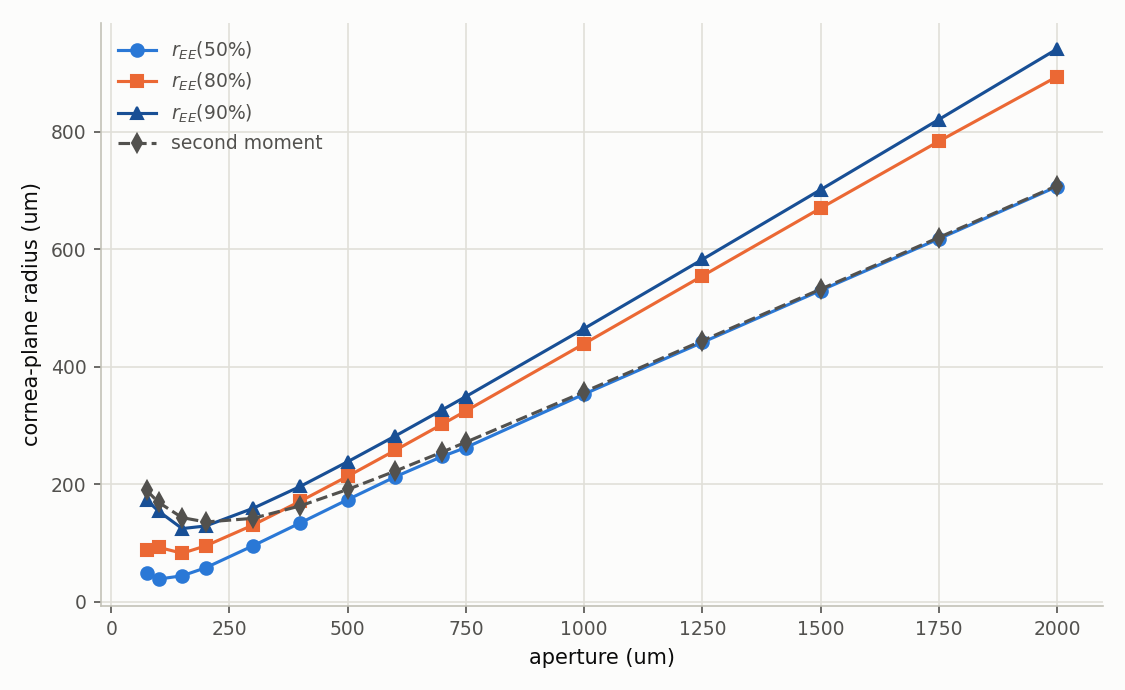
\includegraphics[width=0.85\textwidth]{figures/fig_stage1_cornea_radii.png}
\caption{Stage 1: cornea-plane effective radii ($r_{EE}(50\%)$, $r_{EE}(80\%)$,
$r_{EE}(90\%)$, second-moment radius) vs.\ pinhole aperture, $12\mm$ gap, $550\,$nm.}
\label{fig:stage1-ee}
\end{figure}

{\small
\begin{longtable}{rrrrrrr}
\caption{Stage 1 cornea-plane sweep, 12mm gap, 550nm.}\label{tab:stage1-full}\\
\toprule
a\_hole (um) & N\_F & regime & r\_EE50 (um) & r\_EE80 (um) & r\_EE90 (um) & 2nd moment (um) \\
\midrule
\endfirsthead
\multicolumn{7}{c}{\tablename\ \thetable\ -- continued}\\
\toprule
a\_hole (um) & N\_F & regime & r\_EE50 (um) & r\_EE80 (um) & r\_EE90 (um) & 2nd moment (um) \\
\midrule
\endhead
\bottomrule
\endfoot
75 & 0.21 & Transition & 48.55 & 87.78 & 173.48 & 189.66 \\
100 & 0.38 & Transition & 38.90 & 92.94 & 154.46 & 169.45 \\
150 & 0.85 & Transition & 44.48 & 82.87 & 124.81 & 143.45 \\
200 & 1.52 & Transition & 58.22 & 95.45 & 129.27 & 136.03 \\
300 & 3.41 & Transition & 95.59 & 130.87 & 159.29 & 142.23 \\
400 & 6.06 & Transition & 134.52 & 171.46 & 196.64 & 163.51 \\
500 & 9.47 & Transition & 174.04 & 213.75 & 238.54 & 191.35 \\
600 & 13.64 & Strong Fresnel & 212.67 & 257.74 & 282.05 & 222.39 \\
700 & 18.56 & Strong Fresnel & 247.50 & 302.38 & 326.82 & 255.08 \\
750 & 21.31 & Strong Fresnel & 262.67 & 324.88 & 349.42 & 271.75 \\
1000 & 37.88 & Strong Fresnel & 353.54 & 439.26 & 465.06 & 357.36 \\
1250 & 59.19 & Strong Fresnel & 441.50 & 554.48 & 582.55 & 444.35 \\
1500 & 85.23 & Strong Fresnel & 529.79 & 669.73 & 701.18 & 531.98 \\
1750 & 116.00 & Strong Fresnel & 617.61 & 783.54 & 820.59 & 619.95 \\
2000 & 151.52 & Strong Fresnel & 706.59 & 893.56 & 940.60 & 708.10 \\
\end{longtable}
}

\textbf{Reading this chapter's results}: cornea-plane blur is monotonically decreasing
with aperture over most of this range (a larger pinhole diffracts less), the opposite
trend from the retina-plane result in Chapter~\ref{ch:stage2} once the eye's own
converging lens and myopic defocus are added --- the retina-plane optimum exists
precisely \emph{because} those two effects (diffraction favoring large apertures,
defocus favoring small ones) trade off against each other, a genuine competition Stage
1 alone cannot show since it stops before the lens.

\chapter{Stage 2 --- Full Retina-Plane Blur Model}
\label{ch:stage2}

\section{Pipeline}

Stage 2 (\texttt{stage2\_fixed/}) extends Stage 1 through the eye: pupil clipping,
thin-lens phase, and a second ASM propagation to the retina, using the axial myopia
model of Chapter~\ref{ch:optical_system}. The full chain, per point $(a_{hole}, M)$:

\begin{enumerate}
\item \textbf{Gap propagation}: ASM-propagate the pinhole field $d_{gap}=12\mm$ to the
  corneal plane (identical to Stage 1's own propagation, reused not re-derived).
\item \textbf{Junction validation}: before the lens is ever applied, check (a) the
  cornea field is finite and carries positive energy; (b) the Matsushima band limit at
  the \emph{target} retina distance $v_r$ suppresses under $5\%$ of propagating energy;
  (c) a diffraction-limited minimum-divergence estimate of the beam at $v_r$ stays
  within $40\%$ of the half-window --- a wraparound risk pre-check. Any point failing
  any check is recorded with its specific failure reason and \emph{never silently
  dropped}.
\item \textbf{Pupil clip}: binary circular clip at diameter $D_{pupil}$.
\item \textbf{Lens phase}: thin-lens transmittance
  $\exp\!\big(-ik(x^2+y^2)/(2f_{eye})\big)$, $k=2\pi/\lambda_{eff}$.
\item \textbf{Retina propagation}: second ASM propagation, distance $v_r=L_{ax}(M)$, at
  the same effective wavelength $\lambda_{eff}$.
\item \textbf{Retinal encircled energy}: $r_{EE}(50\%)$, $r_{EE}(70\%)$,
  $r_{EE}(80\%)$, $r_{EE}(90\%)$, and RMS radius, all per
  Section~\ref{sec:effective-radius}.
\end{enumerate}

\textbf{The effective wavelength.} With \texttt{refractive\_index\_correction=True}
(default), $\lambda_{eff}=\lambda/n'$ --- the vitreous's own reduced wavelength ---
and it must be used identically in \emph{both} the lens-phase step and the
retina-propagation step. Getting this one consistency wrong, silently, for an
extended period of this project's history, is the subject of
Chapter~\ref{ch:physics_audit}.

\section{Validation against the closed-form Airy disk}

At zero defocus ($M=0$, $d_{gap}=0$), $v_r=f_{eye}$ by construction and the retinal
PSF should match the classical Airy-disk closed form. The validation gate compares
$r_{EE}(50\%)$, $r_{EE}(80\%)$, and $r_{EE}(90\%)$ against that closed form at stated
tolerances (2\%, 8\%, 2\% respectively --- the wider $r_{EE}(80\%)$ tolerance reflects
genuine ill-conditioning near the Airy pattern's first null, not a looser standard).
The gate \textbf{passes}, and passes at improved accuracy after the Chapter~\ref{ch:physics_audit}
fix ($r_{EE}(50\%)$ error $1.14\%\to0.30\%$; $r_{EE}(80\%)$ $4.56\%\to0.38\%$;
$r_{EE}(90\%)$ $0.55\%\to0.94\%$).

\section{Unmodeled effects, stated explicitly}
\label{sec:unmodeled}

Four simplifications are deliberately built into this pipeline and documented in one
place (\texttt{phase2\_retina.py}'s own module docstring), so a reader never mistakes
them for oversights:

\begin{enumerate}[label=(E\arabic*)]
\item \textbf{Reduced-eye geometry} (Section~\ref{ch:optical_system}): no anterior
  chamber distance, no cornea/lens power split.
\item \textbf{Grid-captured, not emitted, power normalization}: $r_{EE}(P)$'s
  denominator is the power present on the simulation grid at measurement time, not the
  power originally emitted at the aperture. A separate, additive integrated
  energy-escape estimate is provided (comparing against the aperture's exact analytic
  input power $\pi(a_{hole}/2)^2$) and found negligible ($<0.12\%$) at every tested
  configuration.
\item \textbf{Domain mismatch between $r_{EE}(P)$ and threshold-crossing radii}: the
  former bins to the grid corner, the latter search only the inscribed circle ---
  roughly $1.41\times$ smaller in radius. This matters most at high percentiles.
\item \textbf{No chromatic aberration, no higher-order aberrations, no
  Stiles--Crawford apodization in the core PSF, no finite aperture-membrane
  thickness}: the lens phase is a pure quadratic (defocus-only) term; the pupil mask
  is an infinitely-thin binary 0/1 mask.
\end{enumerate}

None of these were found to change any qualitative conclusion in this report, but all
four are genuine simplifications a reader should carry forward, not assume were
checked away.

\chapter{The Physics Audit: A Real Bug, Found and Fixed}
\label{ch:physics_audit}

This chapter documents the single most consequential correction in this project's
history: a real, confirmed error in how the eye's lens phase and the retina
propagation handled the vitreous's refractive index, found by independent re-derivation
(not merely observed), fixed with a minimal signature-preserving change, and
regression-tested before and after. It moved the project's headline optimum-aperture
number substantially. This chapter states what was wrong, why, and exactly how the
answer changed --- \emph{before} presenting corrected-optics results in the rest of this
report, so a reader is never shown one number without also seeing where it came from.

\section{Item A: the lens-phase / retina-propagation wavelength mismatch}

\textbf{The bug.} With \texttt{refractive\_index\_correction=True}, the retina
propagation (step 5, Chapter~\ref{ch:stage2}) correctly used the reduced effective
wavelength $\lambda_{eff}=\lambda/n'$. The lens-phase step (step 4), \emph{prior to
this fix}, used the raw vacuum wavelength $\lambda$ instead.

\textbf{Why this matters, derived two independent ways.}

\emph{Stationary-phase focus-location argument.} For a lens phase screen
$\exp(-ik_L r^2/(2f))$ followed by propagation at wavenumber $k_{prop}$, the true
geometric focus sits at $z^\ast = f\cdot(k_{prop}/k_L)$. With $k_L$ the vacuum
wavenumber and $k_{prop}=n' k_L$ (from the retina propagation's own correction), the
true focus was at $z^\ast=f_{eye}\cdot n'$, not $f_{eye}$ --- a $\approx 33.6\%$ axial
focus error ($n'=1.336$), \emph{independent of aperture or myopia level}.

\emph{Medium-agnostic optical-path-length argument.} For a refracting system with
object-side index 1 and image-side index $n'$, the correct phase screen is
$\exp(-ik_{vac}\,P\,r^2/2)$ regardless of surrounding media. Substituting
$f_{eye}=n'/P_0$ shows this requires $k=k_{vac}\cdot n'$ in the lens phase ---
exactly $\lambda/n'$, matching the retina propagation's own already-correct
convention.

Both derivations agree with each other, and the project's own separate closed-form
validation gate (\texttt{validation\_gate.py}) had already independently computed
$\lambda_{eff}=\lambda/n'$ for its own comparison --- confirming the correct convention
was known project-wide, simply not consistently threaded through the lens call.

\textbf{The fix.} $\lambda_{eff}$ is now resolved once, at the top of the pipeline
point function, and passed to \emph{both} the lens-phase and retina-propagation steps.

\textbf{Why the zero-defocus validation gate did not catch this (Item D).} At $M=0$,
$d_{gap}=0$, the model sits at exact focus by construction. A pure lens-power scaling
error there partly manifests as the wave's true focus shifting to a different
\emph{plane} rather than as a distortion of the in-focus pattern's \emph{shape} ---
which is specifically what the gate compares against the closed-form Airy formula.
This is documented, not silently left as a blind spot: the gate validates pattern
shape at exact focus and is not sensitive, in general, to a pure focal-plane shift.

\section{Item B: the junction validator's own wavelength}

The pre-check in step 2 (Chapter~\ref{ch:stage2}) received the raw vacuum wavelength
rather than $\lambda_{eff}$, which --- since the Matsushima band limit scales as
$1/\lambda$ --- made the check \emph{more conservative than necessary} (never
incorrectly permissive). Quantified directly: the reported band limit differed by
exactly the $n'$ factor between the two wavelengths, but the actual suppression
fraction was $0.0000\%$ either way across every tested configuration --- so this fix
restores real headroom for future, more demanding configurations without changing any
number in this report's own sweeps.

\section{Item C: previously-unchecked lens-phase sampling}

The lens phase's local spatial frequency grows linearly with radius; requiring less
than $\pi$ radians of phase change per grid pixel (a standard Nyquist criterion) gives
the radius beyond which the sampled phase aliases:
\begin{equation}
r_{max,lens} = \frac{\lambda_{eff}\, f_{eye}}{2\,dx}.
\end{equation}
At this project's default configuration this evaluates to $\approx1564\um$, smaller
than the $2000\um$ pupil radius at every tested aperture (since $r_{max,lens}$ does not
depend on $a_{hole}$ at all). Quantified directly, not assumed: only $0.005\%$
(at $a_{hole}=300\um$) to $0.052\%$ (at $a_{hole}=2000\um$) of cornea-plane energy
lies beyond this radius. Added as a new, non-gating diagnostic rather than a hard
pipeline gate, since gating on it uniformly would reject every point rather than
flagging the ones where it actually matters.

\section{Items E1--E4}

Four further design choices were independently verified true of the actual code and
documented in place --- these are the same four points already listed in
Section~\ref{sec:unmodeled}.

\section{The headline result: the optimum aperture moves substantially}

Table~\ref{tab:audit-before-after} is this project's single most important number: the
blur-only optimum aperture (minimizing $r_{EE}(50\%)$), before and after the Item~A/B
fix, across every myopia level tested.

\begin{table}[htbp]
\centering
\begin{tabular}{rrrrr}
\toprule
$M$ (D) & opt.\ aperture: pre$\to$post & change & $r_{EE}(50\%)$ at opt.: pre$\to$post & change \\
\midrule
1 & $300\to700\um$  & $+133.3\%$ & $23.04\to7.33\um$  & $-68.2\%$ \\
2 & $300\to750\um$  & $+150.0\%$ & $22.65\to8.01\um$  & $-64.6\%$ \\
3 & $300\to600\um$  & $+100.0\%$ & $22.29\to10.57\um$ & $-52.6\%$ \\
4 & $300\to500\um$  & $+66.7\%$  & $21.99\to12.02\um$ & $-45.4\%$ \\
5 & $400\to500\um$  & $+25.0\%$  & $20.83\to13.29\um$ & $-36.2\%$ \\
6 & $400\to400\um$  & $0.0\%$    & $19.79\to14.47\um$ & $-26.9\%$ \\
8 & $400\to400\um$  & $0.0\%$    & $18.16\to17.87\um$ & $-1.6\%$ \\
\bottomrule
\end{tabular}
\caption{Blur-only optimum aperture, before vs.\ after the Item A/B wavelength fix.
Reproduced identically across two independent branches of this project's own history.}
\label{tab:audit-before-after}
\end{table}

\textbf{Reading this table.} The bug's absolute focal-shift error
($f_{eye}(n'-1)\approx7.5\mm$) is independent of $M$, so it is a \emph{large} fraction
of the eye's total defocus budget at low myopia (where the true defocus is small) and
proportionally \emph{negligible} once real axial elongation dominates at high $M$ ---
exactly the pattern the table shows: a $+150\%$ change at $M=2\,$D collapsing to $0\%$
by $M=8\,$D. This is physically coherent, not noise: the same qualitative pattern was
independently reproduced on a separate branch of this project's history before being
re-confirmed here.

One further observation, stated plainly and not overinterpreted: the corrected optimum
($400$--$750\um$) sits closer to the independently-derived brightness-constrained
optimum ($900$--$1250\um$, Chapter~\ref{ch:stage3a}) and the clinical bracket
($940$--$1750\um$) than the pre-fix figure did. This narrows part of the gap the
brightness-floor analysis was built to explain, but does not close it.

\textbf{A second, independent bug, found while investigating this one.} A Python
import-order bug meant that two of this project's own acuity-validation efforts
(Chapters~\ref{ch:r7acuity}--\ref{ch:validation}) had, for an extended period, silently
never actually run against this corrected pipeline at all --- see
Chapter~\ref{ch:validation} for the full account and the re-run results.

Every number in every remaining chapter of this report reflects the corrected optics
described here.

\chapter{The R1 Sweep: Corrected-Optics Blur-Only Optimum}
\label{ch:r1sweep}

This chapter presents the full corrected-optics blur-minimization sweep --- this
project's headline result --- across the complete $15\times8$ grid, with no brightness
or acuity constraint applied (Chapters~\ref{ch:stage3a} and~\ref{ch:acuity_models} add
those separately). \textbf{Every result in this chapter is computed and shown for all
four encircled-energy percentiles the pipeline reports at every point} ---
$r_{EE}(50\%)$, $r_{EE}(70\%)$, $r_{EE}(80\%)$, and $r_{EE}(90\%)$
(Section~\ref{sec:effective-radius}) --- not for $r_{EE}(50\%)$ alone.

\section{All four percentiles, full grid}
\label{sec:r1-all-percentiles}

Figure~\ref{fig:r1-lines-all} shows blur vs.\ aperture, one panel per percentile, one
line per myopia level within each panel. Every curve at every percentile is
U-shaped: diffraction dominates at small apertures (blur decreases as the aperture
grows), while defocus dominates at large apertures (blur increases again as more of
the eye's uncorrected myopic power is exposed) --- the aperture-size trade-off this
whole report is built around, and a shape that holds regardless of which percentile is
used. Figure~\ref{fig:r1-heatmap-all} shows the identical data as four
aperture$\times$$M$ heatmaps.

\begin{figure}[htbp]
\centering
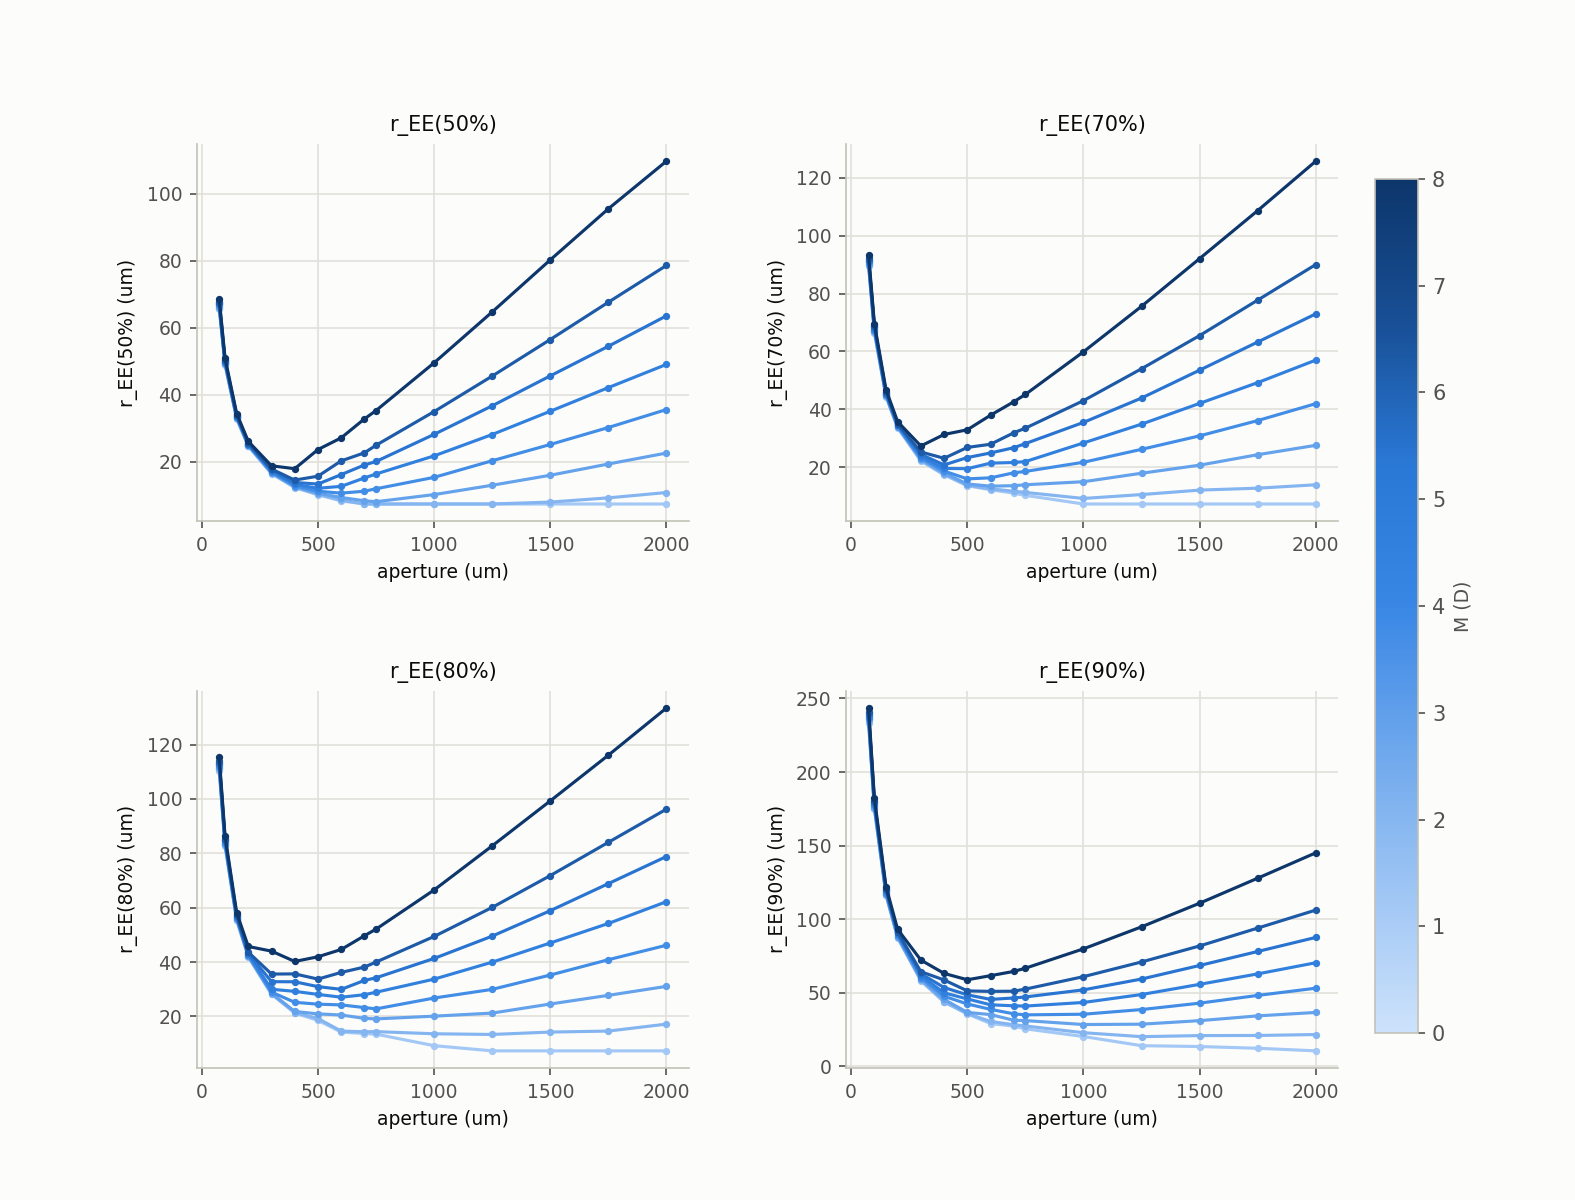
\includegraphics[width=\textwidth]{figures/fig_r1_lines_all_percentiles.png}
\caption{Corrected-optics blur vs.\ aperture, all four percentiles, one line per myopia level $M$ within each panel (sequential blue colormap, darker = higher $M$).}
\label{fig:r1-lines-all}
\end{figure}

\begin{figure}[htbp]
\centering
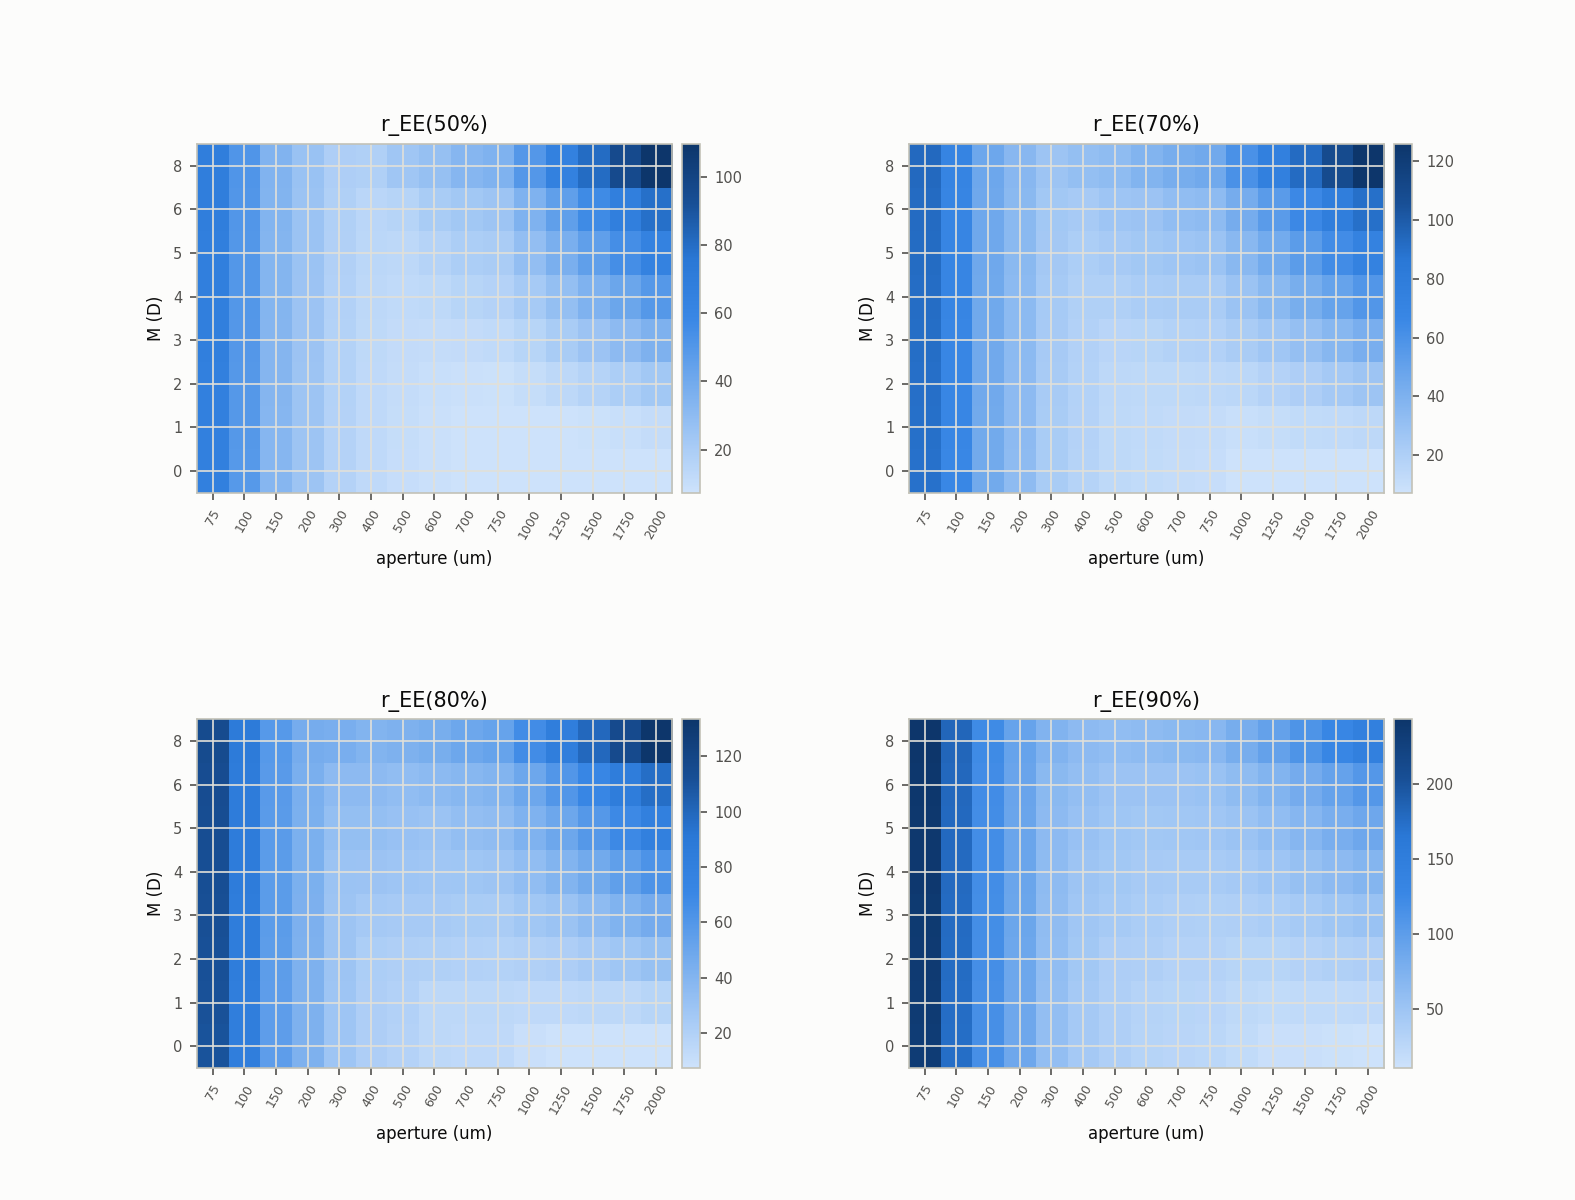
\includegraphics[width=\textwidth]{figures/fig_r1_heatmap_all_percentiles.png}
\caption{Corrected-optics blur (\textmu m) across the full aperture $\times$ myopia grid, all four percentiles.}
\label{fig:r1-heatmap-all}
\end{figure}

{\small
\begin{longtable}{rrrrr}
\caption{Unconstrained blur-only optimal aperture (um), all four percentiles, per myopia level.}\label{tab:r1-all-percentiles}\\
\toprule
M (D) & r\_EE(50\%) & r\_EE(70\%) & r\_EE(80\%) & r\_EE(90\%) \\
\midrule
\endfirsthead
\multicolumn{5}{c}{\tablename\ \thetable\ -- continued}\\
\toprule
M (D) & r\_EE(50\%) & r\_EE(70\%) & r\_EE(80\%) & r\_EE(90\%) \\
\midrule
\endhead
\bottomrule
\endfoot
0 & 700 & 1000 & 1250 & 2000 \\
1 & 700 & 1000 & 1250 & 1250 \\
2 & 750 & 600 & 750 & 1000 \\
3 & 600 & 500 & 750 & 750 \\
4 & 500 & 500 & 600 & 750 \\
5 & 500 & 400 & 600 & 600 \\
6 & 400 & 400 & 500 & 600 \\
8 & 400 & 300 & 400 & 500 \\
\end{longtable}
}

The optimal aperture is not the same number across percentiles, and the choice
matters: at $M=8\,$D it ranges from $300\um$ ($r_{EE}(70\%)$) to $500\um$
($r_{EE}(90\%)$) --- a $67\%$ spread from changing only which fraction of encircled
energy is minimized, with no other assumption changed at all.
\textbf{Important caveat, carried forward from this exact table}: the $M=0$ and
$M=1$ columns for $r_{EE}(70\%)$ and $r_{EE}(80\%)$ are not genuine unique minima ---
Chapter~\ref{ch:percentile} identifies and quantifies a grid-resolution saturation
artifact at those two myopia levels specifically, and should be read before treating
those two rows at face value. $M\ge2$ rows are unaffected and trustworthy.

\section{The $r_{EE}(50\%)$ case in detail}

$r_{EE}(50\%)$ is this project's historically primary metric (it is what
Chapter~\ref{ch:physics_audit}'s own audit was originally measured against) and is
worth walking through on its own as the anchoring case before the cross-percentile
comparison above. Table~\ref{tab:r1-optimum} restates its column from
Table~\ref{tab:r1-all-percentiles} alone, for reference alongside the discussion below.

{\small
\begin{longtable}{rrr}
\caption{Blur-only optimal aperture per myopia level, corrected optics.}\label{tab:r1-optimum}\\
\toprule
M (D) & optimal aperture (um) & r\_EE(50\%) at optimum (um) \\
\midrule
\endfirsthead
\multicolumn{3}{c}{\tablename\ \thetable\ -- continued}\\
\toprule
M (D) & optimal aperture (um) & r\_EE(50\%) at optimum (um) \\
\midrule
\endhead
\bottomrule
\endfoot
0.00 & 700.00 & 7.33 \\
1.00 & 700.00 & 7.33 \\
2.00 & 750.00 & 8.01 \\
3.00 & 600.00 & 10.57 \\
4.00 & 500.00 & 12.02 \\
5.00 & 500.00 & 13.29 \\
6.00 & 400.00 & 14.47 \\
8.00 & 400.00 & 17.87 \\
\end{longtable}
}

\section{Reading the result}

The blur-only optimum aperture is smallest at low myopia ($400$--$750\um$ for
$M\le5\,$D by $r_{EE}(50\%)$) and shrinks further at high myopia ($400\um$ by
$M=6$--$8\,$D) --- more myopia means more inherent defocus at any fixed aperture, so
the optimum shifts toward apertures small enough to suppress that defocus
geometrically, even at the cost of more diffraction. This is the single physically
intuitive result underlying the whole ``pinhole helps myopia'' effect: a smaller
aperture increases depth of focus by geometric blur reduction faster than it worsens
diffraction blur, up to the point where diffraction itself starts to dominate. The
same qualitative statement holds at every percentile (Figure~\ref{fig:r1-lines-all}),
only the exact optimal aperture number shifts (Table~\ref{tab:r1-all-percentiles}).

\textbf{This optimum, on its own, is not the design recommendation this report ends
with.} At every percentile, it systematically favors apertures well below the
clinically observed range ($940$--$1750\um$, per this project's own patent/literature
cross-reference) and below what any brightness constraint would tolerate --- exactly
the gap Chapter~\ref{ch:stage3a} exists to explain, again at every percentile.

\chapter{Stage 3a --- Brightness-Constrained Optimum}
\label{ch:stage3a}

\section{Motivation}

Chapter~\ref{ch:r1sweep}'s pure blur-minimization optimum sits well below the range
sunglasses manufacturers and patent filings actually use. Stage 3a asks: does adding a
single, simple brightness (illuminance) floor to the optimization --- \emph{minimize
blur, subject to admitting at least a minimum fraction of full-pupil light} --- close
that gap?

\section{Relative illuminance}

For a single circular pinhole of diameter $a_{hole}$ in front of an eye with natural
(unobstructed) pupil diameter $D_{pupil}$, diffraction redistributes power spatially
but does not destroy it: total transmitted power through the aperture is proportional
to its physical area, not to any diffraction-broadened blur-radius estimate. Once
$a_{hole}$ exceeds $D_{pupil}$, the pupil itself becomes the limiting stop. Relative
illuminance (as a fraction of normal, full-pupil viewing) is therefore the clipped
area ratio
\begin{equation}
E_{rel}(a_{hole}) = \left(\frac{\min(a_{hole}, D_{pupil})}{D_{pupil}}\right)^{2}.
\label{eq:erel}
\end{equation}

\section{The constrained optimization}

For each myopia level $M$, Stage 3a takes the full corrected-optics blur sweep
(Chapter~\ref{ch:r1sweep}), restricts to apertures with $E_{rel}(a_{hole}) \ge T_{min}$,
and reports the aperture within that restricted set that minimizes $r_{EE}(50\%)$ ---
i.e., the smallest-blur aperture that still clears the brightness floor. This report
uses $T_{min}=6.25\%$, the low end of this project's own previously-established
brightness-floor range ($6.25$--$9\%$).

\begin{figure}[htbp]
\centering
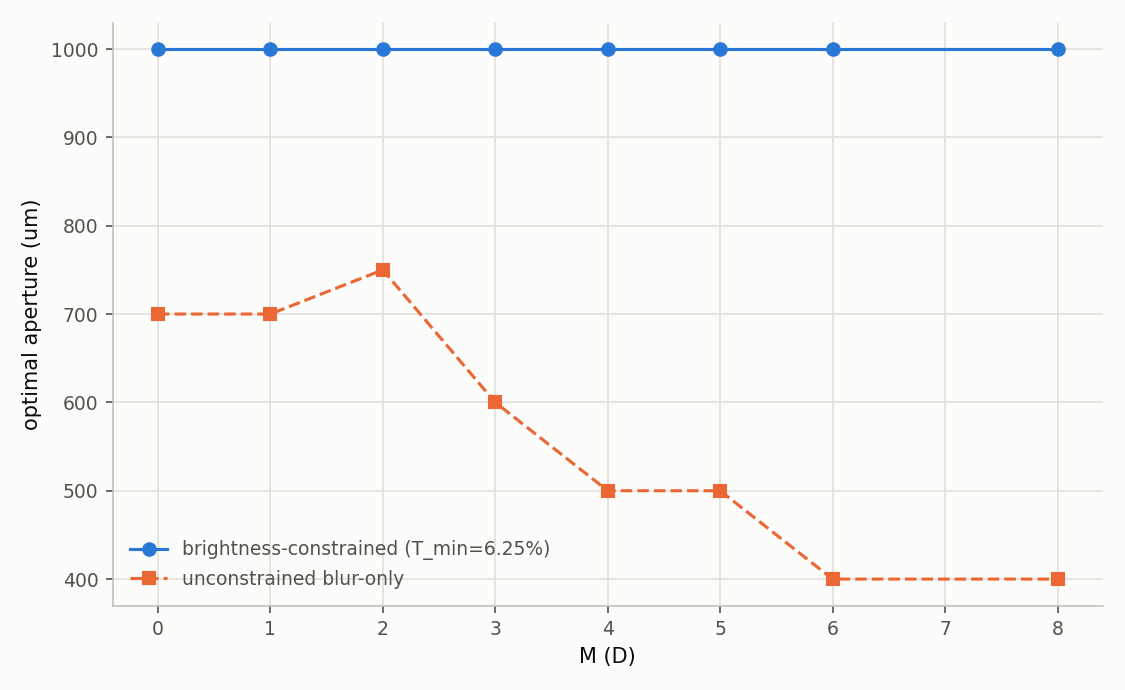
\includegraphics[width=0.85\textwidth]{figures/fig_stage3a_optimum_vs_M.png}
\caption{Brightness-constrained optimum aperture $a^\ast$ vs.\ myopia $M$, $T_{min}=6.25\%$, alongside the unconstrained (Chapter~\ref{ch:r1sweep}) optimum for comparison.}
\label{fig:stage3a-optimum}
\end{figure}

{\small
\begin{longtable}{rrrrr}
\caption{Brightness-constrained optimum, T\_min=6.25\%.}\label{tab:stage3a-full}\\
\toprule
M (D) & T\_min & a* (um) & r\_EE(50\%) at a* (um) & E\_rel at a* \\
\midrule
\endfirsthead
\multicolumn{5}{c}{\tablename\ \thetable\ -- continued}\\
\toprule
M (D) & T\_min & a* (um) & r\_EE(50\%) at a* (um) & E\_rel at a* \\
\midrule
\endhead
\bottomrule
\endfoot
0.0000 & 0.0625 & 1000.0000 & 7.3275 & 0.0625 \\
1.0000 & 0.0625 & 1000.0000 & 7.3275 & 0.0625 \\
2.0000 & 0.0625 & 1000.0000 & 10.1398 & 0.0625 \\
3.0000 & 0.0625 & 1000.0000 & 15.2893 & 0.0625 \\
4.0000 & 0.0625 & 1000.0000 & 21.7056 & 0.0625 \\
5.0000 & 0.0625 & 1000.0000 & 28.1338 & 0.0625 \\
6.0000 & 0.0625 & 1000.0000 & 34.9404 & 0.0625 \\
8.0000 & 0.0625 & 1000.0000 & 49.5132 & 0.0625 \\
\end{longtable}
}

\section{Result}

A single brightness floor of $6.25\%$ of full-pupil illuminance moves the optimum from
the unconstrained $400$--$750\um$ bracket ($r_{EE}(50\%)$, $M\le5\,$D) to $1000\um$ ---
much closer to the clinically observed bracket.

\textbf{An important caveat about the floor value itself, stated plainly.} The
$6.25$--$9\%$ figure was originally \emph{reverse-engineered} to reproduce the known
clinical range, not independently derived from a cited absolute-brightness threshold.
Chapter~\ref{ch:brightness_reconciliation} attempts exactly that independent
reconciliation, and reports it as still only partially resolved.

\section{All four blur percentiles under the same brightness constraint}
\label{sec:stage3a-all-percentiles}

Repeating this exact constrained optimization for $r_{EE}(70\%)$, $r_{EE}(80\%)$, and
$r_{EE}(90\%)$ --- at this same spot, using the identical $T_{min}=6.25\%$ floor and
the identical selection rule (smallest $r_{EE}(P)$ among apertures clearing the floor)
--- gives Figure~\ref{fig:stage3a-all-percentiles} and
Table~\ref{tab:stage3a-all-percentiles}.

\begin{figure}[htbp]
\centering
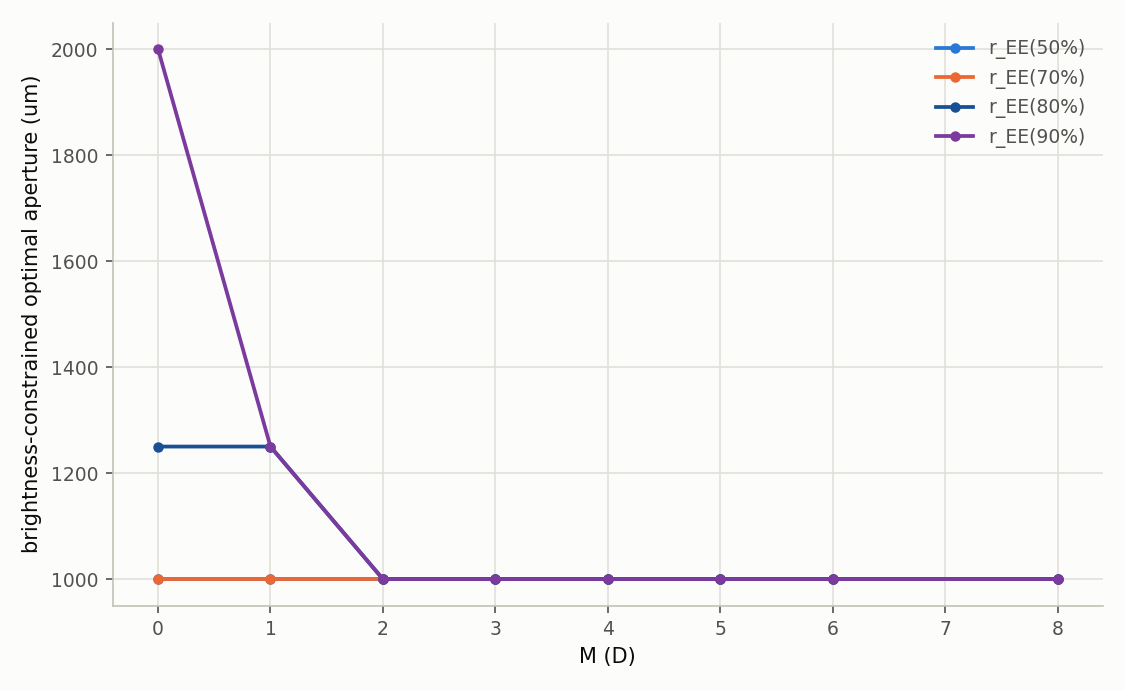
\includegraphics[width=0.85\textwidth]{figures/fig_stage3a_all_percentiles.png}
\caption{Brightness-constrained optimal aperture vs.\ myopia, all four blur percentiles, $T_{min}=6.25\%$.}
\label{fig:stage3a-all-percentiles}
\end{figure}

{\small
\begin{longtable}{rrrrr}
\caption{Brightness-constrained optimal aperture (um, T\_min=6.25\%), all four percentiles, per myopia level.}\label{tab:stage3a-all-percentiles}\\
\toprule
M (D) & r\_EE(50\%) & r\_EE(70\%) & r\_EE(80\%) & r\_EE(90\%) \\
\midrule
\endfirsthead
\multicolumn{5}{c}{\tablename\ \thetable\ -- continued}\\
\toprule
M (D) & r\_EE(50\%) & r\_EE(70\%) & r\_EE(80\%) & r\_EE(90\%) \\
\midrule
\endhead
\bottomrule
\endfoot
0 & 1000 & 1000 & 1250 & 2000 \\
1 & 1000 & 1000 & 1250 & 1250 \\
2 & 1000 & 1000 & 1000 & 1000 \\
3 & 1000 & 1000 & 1000 & 1000 \\
4 & 1000 & 1000 & 1000 & 1000 \\
5 & 1000 & 1000 & 1000 & 1000 \\
6 & 1000 & 1000 & 1000 & 1000 \\
8 & 1000 & 1000 & 1000 & 1000 \\
\end{longtable}
}

\textbf{A clean, generalizable finding, not visible from $r_{EE}(50\%)$ alone}: for
$M\ge2\,$D, \emph{all four percentiles converge to exactly the same optimal aperture}
($1000\um$) --- the brightness floor itself, not any property of the blur curve. This
is a direct, mechanical consequence of how the constrained search works: once the
\emph{unconstrained} optimum for a given percentile (Table~\ref{tab:r1-all-percentiles},
Section~\ref{sec:r1-all-percentiles}) already sits \emph{below} the floor aperture
($1000\um$ at $T_{min}=6.25\%$, $D_{pupil}=4000\um$), the constrained search is pushed
outward along the (still-decreasing, then floor-clipped) blur curve until it reaches
the floor itself and stops there --- so \emph{whenever the floor binds, which
percentile you optimize stops mattering entirely}. This only fails to hold at
$M=0$--$1\,$D, where $r_{EE}(80\%)$'s and $r_{EE}(90\%)$'s own \emph{unconstrained}
optima already sit at or above the floor (Table~\ref{tab:r1-all-percentiles}), so the
brightness constraint never binds for them and the constrained optimum simply equals
the unconstrained one.

\textbf{Practical reading}: at the myopia levels this project's own literature review
identifies as the clinically relevant range (moderate-to-high, $M\ge2\,$D), the choice
of blur-percentile metric --- one of this report's own recurring caveats
(Chapter~\ref{ch:percentile}) --- turns out not to matter for the brightness-constrained
design number at all, \emph{provided} the $6.25\%$ floor itself is trusted. The
remaining open question is therefore squarely the floor value, not the blur metric ---
exactly what Chapter~\ref{ch:brightness_reconciliation} investigates next.

\chapter{Brightness Reconciliation: Absolute vs.\ Percentage Thresholds}
\label{ch:brightness_reconciliation}

\section{Two independently-derived thresholds that had never been checked against each other}

Chapter~\ref{ch:stage3a}'s $6.25$--$9\%$ brightness floor is a \emph{relative}
(percentage) threshold, reverse-engineered to match the clinical bracket. A separate
literature review (independent of Stage 3a) identified two \emph{absolute} photometric
thresholds with real citations:

\begin{itemize}
\item \textbf{Van Nes \& Bouman (1967)}: a strict Weber/de~Vries--Rose transition at
  $300$ photopic trolands (Td) --- contrast threshold is illuminance-independent
  (Weber--Fechner) above this level, and scales as $\text{Td}^{-0.5}$ below it.
\item \textbf{CIE 191:2010}: a more permissive photopic/mesopic adapting-luminance
  boundary, $3$--$5\,\text{cd/m}^2$.
\end{itemize}

This chapter reconciles the two, using the same troland formula used throughout this
project:
\begin{equation}
\text{Td} = L_{scene}\;[\text{cd/m}^2] \times A_{aperture}\;[\text{mm}^2], \qquad
A_{aperture}=\pi\left(\frac{a_{hole}}{2}\right)^2 [\text{mm}^2].
\label{eq:troland}
\end{equation}
Inverting Equation~\eqref{eq:troland} for the minimum aperture that clears a given Td
floor at a given scene luminance:
\begin{equation}
a_{min}(\text{Td}_{floor}, L_{scene}) = 2000\sqrt{\frac{\text{Td}_{floor}}{\pi\, L_{scene}}}\;\;[\um].
\end{equation}

\begin{figure}[htbp]
\centering
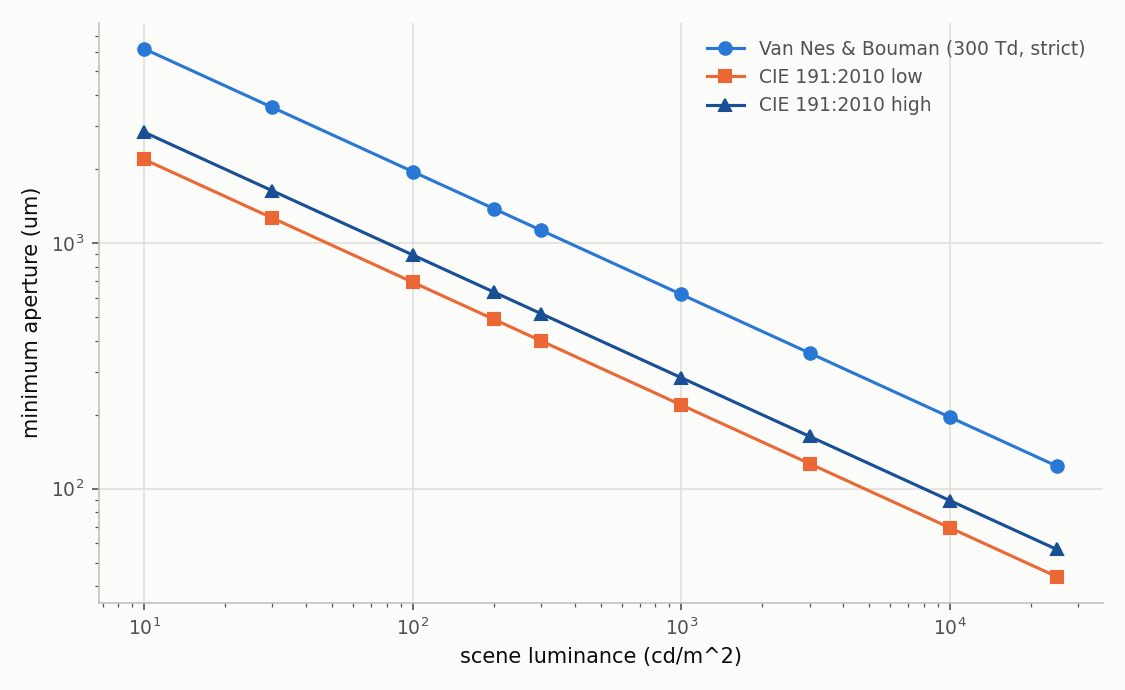
\includegraphics[width=0.85\textwidth]{figures/fig_brightness_reconciliation.png}
\caption{Minimum aperture clearing each absolute threshold (Van~Nes \& Bouman $300$\,Td; CIE 191:2010 $37.7$--$62.8$\,Td-equivalent), vs.\ scene luminance.}
\label{fig:brightness-reconciliation}
\end{figure}

{\small
\begin{longtable}{rrrr}
\caption{Minimum aperture clearing each absolute brightness threshold, vs. scene luminance.}\label{tab:brightness-full}\\
\toprule
scene lum (cd/m2) & min aperture, CIE low (um) & min aperture, CIE high (um) & min aperture, VN\&B (um) \\
\midrule
\endfirsthead
\multicolumn{4}{c}{\tablename\ \thetable\ -- continued}\\
\toprule
scene lum (cd/m2) & min aperture, CIE low (um) & min aperture, CIE high (um) & min aperture, VN\&B (um) \\
\midrule
\endhead
\bottomrule
\endfoot
10.0 & 2190.9 & 2828.4 & 6180.4 \\
30.0 & 1264.9 & 1633.0 & 3568.2 \\
100.0 & 692.8 & 894.4 & 1954.4 \\
200.0 & 489.9 & 632.5 & 1382.0 \\
300.0 & 400.0 & 516.4 & 1128.4 \\
1000.0 & 219.1 & 282.8 & 618.0 \\
3000.0 & 126.5 & 163.3 & 356.8 \\
10000.0 & 69.3 & 89.4 & 195.4 \\
25000.0 & 43.8 & 56.6 & 123.6 \\
\end{longtable}
}

\section{Result: the thresholds only agree at one specific scene luminance}

The two thresholds --- the Stage 3a reverse-engineered percentage floor and the
absolute troland floors above --- only coincide at a specific assumed scene/chart
luminance, and that luminance is \emph{not} this project's own default
($10{,}000\,\text{cd/m}^2$, bright daylight, used throughout the Stage 3/4 acuity
sweeps in Chapters~\ref{ch:stage4}--\ref{ch:validation}). This is an open item, stated
plainly: the two thresholds are not yet fully reconciled against each other, and doing
so is flagged in Chapter~\ref{ch:limitations} as one of this project's highest-value
remaining tasks, precisely because both pieces of code already exist and simply had
never been run against each other before this chapter.

\chapter{Single-Hole Illumination}
\label{ch:singleilluminate}

\texttt{singleilluminate/} provides the unified illumination interface for this
project's single-hole case (its multi-hole array extension is explicitly out of scope
for this report --- see Chapter~\ref{ch:introduction}). It reuses
Equation~\eqref{eq:erel} directly, cross-checked at import time against
\texttt{photometry.py}'s independently-implemented version of the same formula (both
must agree to $10^{-12}$ relative tolerance, checked automatically, or the module
refuses to run) --- a real, executable consistency check between two independently
written implementations of the same physical relationship, not merely a documented
claim that they agree.

\begin{figure}[htbp]
\centering
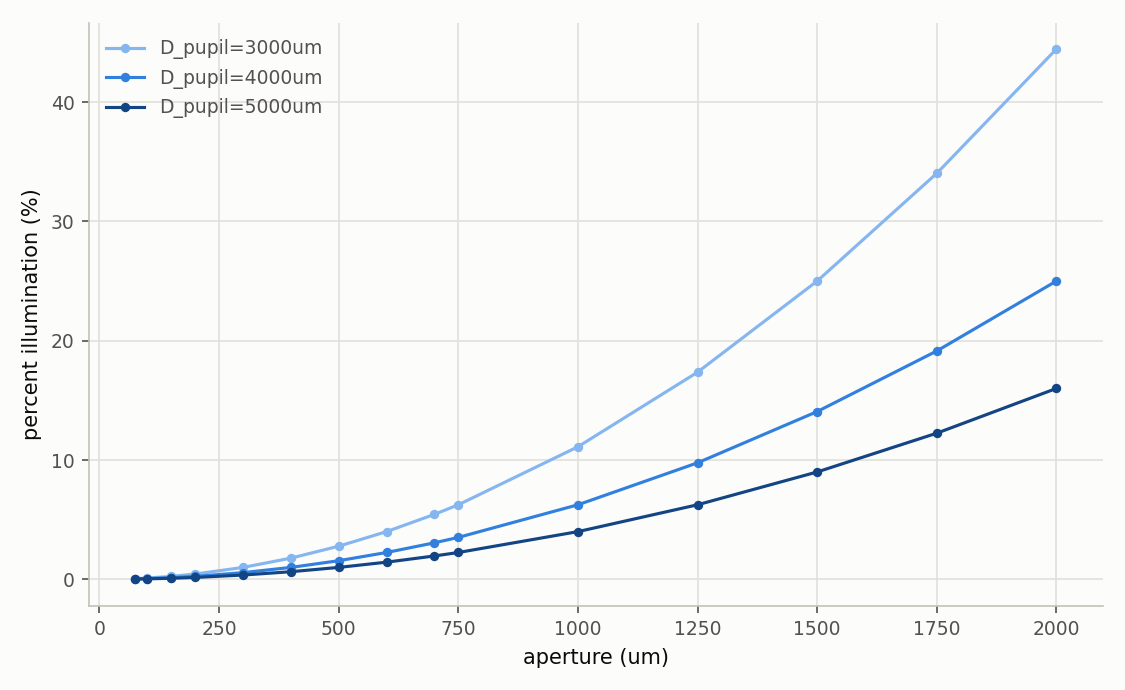
\includegraphics[width=0.85\textwidth]{figures/fig_singleilluminate.png}
\caption{Percent illumination vs.\ aperture, for three natural pupil diameters (3, 4, 5\,mm).}
\label{fig:singleilluminate}
\end{figure}

{\small
\begin{longtable}{rrr}
\caption{Single-hole percent illumination vs. aperture and natural pupil diameter.}\label{tab:singleilluminate-full}\\
\toprule
a\_hole (um) & D\_pupil (um) & percent illumination (\%) \\
\midrule
\endfirsthead
\multicolumn{3}{c}{\tablename\ \thetable\ -- continued}\\
\toprule
a\_hole (um) & D\_pupil (um) & percent illumination (\%) \\
\midrule
\endhead
\bottomrule
\endfoot
75.000 & 3000.000 & 0.062 \\
100.000 & 3000.000 & 0.111 \\
150.000 & 3000.000 & 0.250 \\
200.000 & 3000.000 & 0.444 \\
300.000 & 3000.000 & 1.000 \\
400.000 & 3000.000 & 1.778 \\
500.000 & 3000.000 & 2.778 \\
600.000 & 3000.000 & 4.000 \\
700.000 & 3000.000 & 5.444 \\
750.000 & 3000.000 & 6.250 \\
1000.000 & 3000.000 & 11.111 \\
1250.000 & 3000.000 & 17.361 \\
1500.000 & 3000.000 & 25.000 \\
1750.000 & 3000.000 & 34.028 \\
2000.000 & 3000.000 & 44.444 \\
75.000 & 4000.000 & 0.035 \\
100.000 & 4000.000 & 0.062 \\
150.000 & 4000.000 & 0.141 \\
200.000 & 4000.000 & 0.250 \\
300.000 & 4000.000 & 0.562 \\
400.000 & 4000.000 & 1.000 \\
500.000 & 4000.000 & 1.562 \\
600.000 & 4000.000 & 2.250 \\
700.000 & 4000.000 & 3.062 \\
750.000 & 4000.000 & 3.516 \\
1000.000 & 4000.000 & 6.250 \\
1250.000 & 4000.000 & 9.766 \\
1500.000 & 4000.000 & 14.062 \\
1750.000 & 4000.000 & 19.141 \\
2000.000 & 4000.000 & 25.000 \\
75.000 & 5000.000 & 0.022 \\
100.000 & 5000.000 & 0.040 \\
150.000 & 5000.000 & 0.090 \\
200.000 & 5000.000 & 0.160 \\
300.000 & 5000.000 & 0.360 \\
400.000 & 5000.000 & 0.640 \\
500.000 & 5000.000 & 1.000 \\
600.000 & 5000.000 & 1.440 \\
700.000 & 5000.000 & 1.960 \\
750.000 & 5000.000 & 2.250 \\
1000.000 & 5000.000 & 4.000 \\
1250.000 & 5000.000 & 6.250 \\
1500.000 & 5000.000 & 9.000 \\
1750.000 & 5000.000 & 12.250 \\
2000.000 & 5000.000 & 16.000 \\
\end{longtable}
}

As expected from Equation~\eqref{eq:erel}, percent illumination grows quadratically
with aperture up to $a_{hole}=D_{pupil}$ and saturates at $100\%$ beyond it; a larger
natural pupil shifts the saturation point outward and lowers percent illumination at
any fixed aperture below it, since the same physical aperture area represents a
smaller fraction of a larger pupil's area.

\chapter{Optical Quality Metrics: MTF, OTF, and the Strehl Ratio}
\label{ch:mtf_strehl}

Stage 3 (\texttt{stage3\_human\_vision/}) adds a battery of standard optical-quality
metrics on top of Stage 2's retinal PSF, as the bridge into the human-vision models of
Chapters~\ref{ch:csf}--\ref{ch:stage4}.

\section{MTF and OTF from the PSF}

The complex optical transfer function is the normalized Fourier transform of the PSF,
radially averaged into 1-D:
\begin{equation}
\text{OTF}(f) = \frac{\big\langle \mathcal{F}\{I(x,y)\}\big\rangle_{|f_x,f_y|=f}}
{\mathcal{F}\{I\}(0,0)}, \qquad \text{MTF}(f)=|\text{OTF}(f)|.
\end{equation}
Retina-plane spatial frequency (cycles/\textmu m) converts to the clinically standard
cycles/degree of visual angle via the eye's own posterior nodal distance $v_r$
(small-angle approximation): $1^\circ$ subtends $v_r\tan(1^\circ)\approx v_r\,(\pi/180)$
at the retina. MTF50 and MTF10 (the frequencies at which MTF drops to $50\%$ and
$10\%$ of its DC value) are reported as two candidate resolution-limit criteria.

\section{Strehl ratio}

\begin{equation}
S = \frac{I_{peak,actual}/P_{actual}}{I_{peak,DL}/P_{DL}}
\end{equation}
comparing peak PSF intensity (each normalized by its own total power first) against a
diffraction-limited reference --- \textbf{this project's fixed convention: the same
system's own $M=0$ (zero-defocus, emmetropic) PSF at the same $(a_{hole}, \lambda,
d_{gap})$}, not an idealized Airy disk.

\subsection*{Finding: the Strehl ratio is not well-posed in this near-field regime}

A direct numerical scan of peak retinal intensity vs.\ propagation distance $v_r$, at
fixed $a_{hole}=750\um$, found peak intensity is \textbf{not} single-peaked in $v_r$ ---
it oscillates, the same near-field Fresnel behavior as Stage 1's own on-axis
oscillation formula (Chapter~\ref{ch:stage1}). Concretely, that scan found a peak of
$1239$ (a.u.) at $v_r=29\mm$, against only $\approx76$--$77$ at $v_r=23$--$25\mm$ ---
precisely where $M=4$--$5\,$D actually places the retina. \textbf{This means $M=0$ is
demonstrably not always the true best-focus condition}, so Strehl computed against the
$M=0$ reference \emph{can legitimately exceed $1.0$} for some $(a_{hole}, M)$
combinations --- confirmed directly in this report's own sweeps (Figure~\ref{fig:strehl-heatmap}),
reaching values as high as $\approx3.7$ at $M=8\,$D. This is not a code bug; it is a
property of operating in the Fresnel near-field regime ($N_F\gtrsim1$), where the
classical Strehl ratio --- built for mildly-aberrated, near-diffraction-limited systems
with one well-defined focus --- is not a well-posed metric. Every chapter downstream
that reports Strehl explicitly carries this caveat rather than treating
Strehl-exceeds-unity points as errors.

\begin{figure}[htbp]
\centering
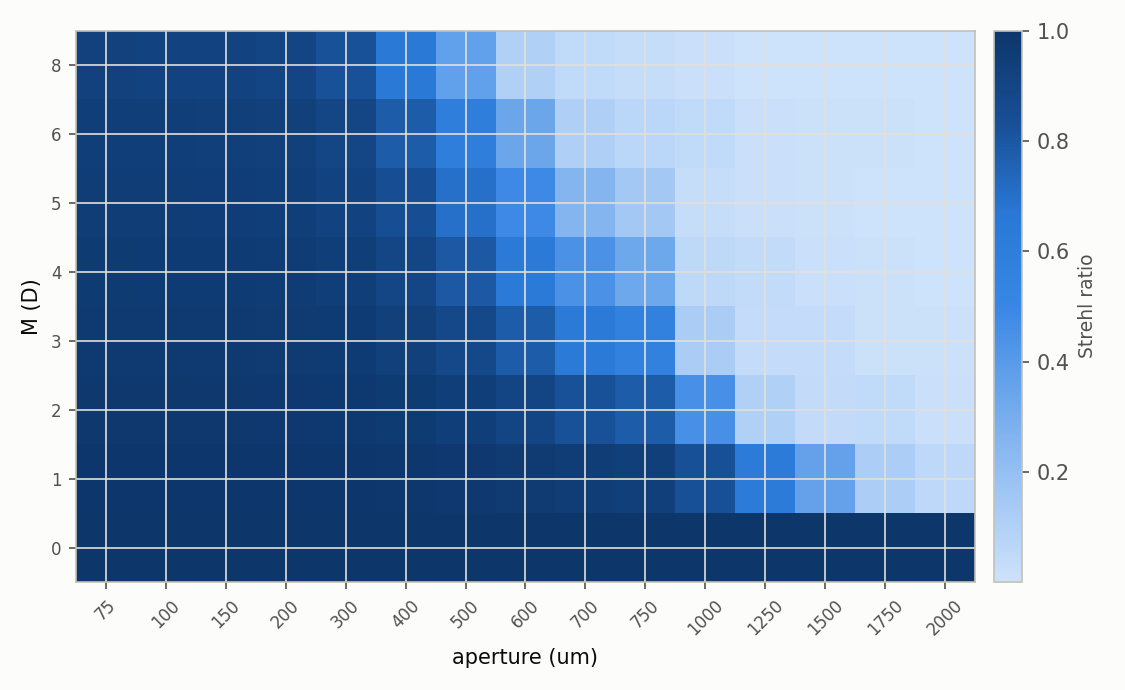
\includegraphics[width=0.85\textwidth]{figures/fig_strehl_heatmap.png}
\caption{Strehl ratio across the full aperture $\times$ myopia grid --- note values exceeding 1.0 at high $M$, a genuine near-field effect, not an artifact.}
\label{fig:strehl-heatmap}
\end{figure}

\section{A related, similarly unstable metric: FWHM}

FWHM (Section~\ref{sec:effective-radius}) is subject to the same ring-hopping
instability documented at the corneal plane in Stage 1 --- and confirmed \emph{worse}
at the retina plane, where the profile's peak/crossing point can hop between Fresnel
rings for adjacent aperture values only a few microns apart. Every FWHM value reported
anywhere in this project's sweeps carries its crossing mode and crossing count
alongside the radius, specifically so an unstable reading is visible rather than
silently trusted as a clean number. \textbf{Neither Strehl nor FWHM should be used as a
primary design metric in this regime without further work} --- $r_{EE}(P)$ and RMS
radius, which integrate over structure rather than reading one potentially-lucky peak
or crossing, are preferred throughout this report.

{\small
\begin{longtable}{rrrrrr}
\caption{Stage 3 optical-quality metrics at aperture=750um, all myopia levels.}\label{tab:mtf-strehl-full}\\
\toprule
M (D) & MTF50 (cpd) & MTF10 (cpd) & Strehl & Strehl>1 & RMS radius (um) \\
\midrule
\endfirsthead
\multicolumn{6}{c}{\tablename\ \thetable\ -- continued}\\
\toprule
M (D) & MTF50 (cpd) & MTF10 (cpd) & Strehl & Strehl>1 & RMS radius (um) \\
\midrule
\endhead
\bottomrule
\endfoot
0.000 & 12.840 & 25.597 & 1.000 & False & 82.924 \\
1.000 & 11.993 & 25.773 & 0.937 & False & 83.439 \\
2.000 & 9.548 & 25.558 & 0.778 & False & 84.222 \\
3.000 & 7.138 & 23.944 & 0.559 & False & 85.294 \\
4.000 & 5.510 & 12.892 & 0.333 & False & 86.675 \\
5.000 & 4.445 & 8.918 & 0.149 & False & 88.382 \\
6.000 & 3.712 & 6.941 & 0.071 & False & 90.433 \\
8.000 & 2.784 & 4.862 & 0.032 & False & 95.626 \\
\end{longtable}
}

\chapter{Contrast Sensitivity Function Models}
\label{ch:csf}

Predicting acuity from an optical MTF requires weighting it by the human visual
system's own contrast sensitivity function (CSF) --- how sensitive the neural pathway
itself is to contrast at each spatial frequency, independent of the eye's optics. This
project uses three CSF parametrizations of deliberately different fidelity, and is
careful to always label which one produced a given number.

\section{Heuristic log-parabola models}

Two simplified, peak-location-matched log-parabola curves, normalized to $1$ at a
stated peak frequency $f_{peak}$:
\begin{equation}
\text{CSF}(f) = \exp\!\left(-\frac{(\log_2(f/f_{peak}))^2}{2\sigma^2}\right), \qquad
\sigma = \frac{\text{bandwidth (octaves)}}{2.355}
\end{equation}
with $f_{peak}=4$\,cpd (``photopic'' variant) or $f_{peak}=8$\,cpd (Mannos--Sakrison
variant). Both are explicitly documented as fit only to peak location and general
band-pass shape, \textbf{not} a full multi-parameter psychophysical model.

\section{The real Barten (1999) model}

A second, independent, luminance- and field-size-dependent CSF is used specifically
where fidelity matters most: R7acuity's neural transfer function
(Chapter~\ref{ch:r7acuity}). Its optical, neural-noise, and eye-movement terms are
\begin{align}
M_{opt}(u) &= e^{-2\pi^2\sigma^2 u^2}, & \sigma &= \sqrt{\sigma_0^2 + (C_{ab}d)^2} \\
M_{as}(u) &= \Big[ \big(X_0^{-2}+X_{max}^{-2}+u^2 N_{max}^{-2}\big)\big(Y_0^{-2}+Y_{max}^{-2}+u^2 N_{max}^{-2}\big)\Big]^{1/2} \\
S(u) &= \frac{M_{opt}(u)/k}{\sqrt{\dfrac{2}{T} M_{as}(u)\left[\dfrac{1}{npE} + \dfrac{\phi_0}{1-e^{-(u/u_0)^2}}\right]}}
\end{align}
with pupil diameter $d$ (Stanley--Davies) and retinal illuminance $E$ (with
Stiles--Crawford correction) both derived from scene luminance and field size. This
implementation is verified bit-for-bit against the published \texttt{colour-science}
open-source library's own doctested reference value
(\texttt{contrast\_sensitivity\_\allowbreak function\_\allowbreak Barten1999(4)} $=360.8691122\ldots$), which
itself cites Barten (1999, 2003) and ITU-R BT.2246-4 --- the highest-fidelity CSF used
anywhere in this project.

\begin{figure}[htbp]
\centering
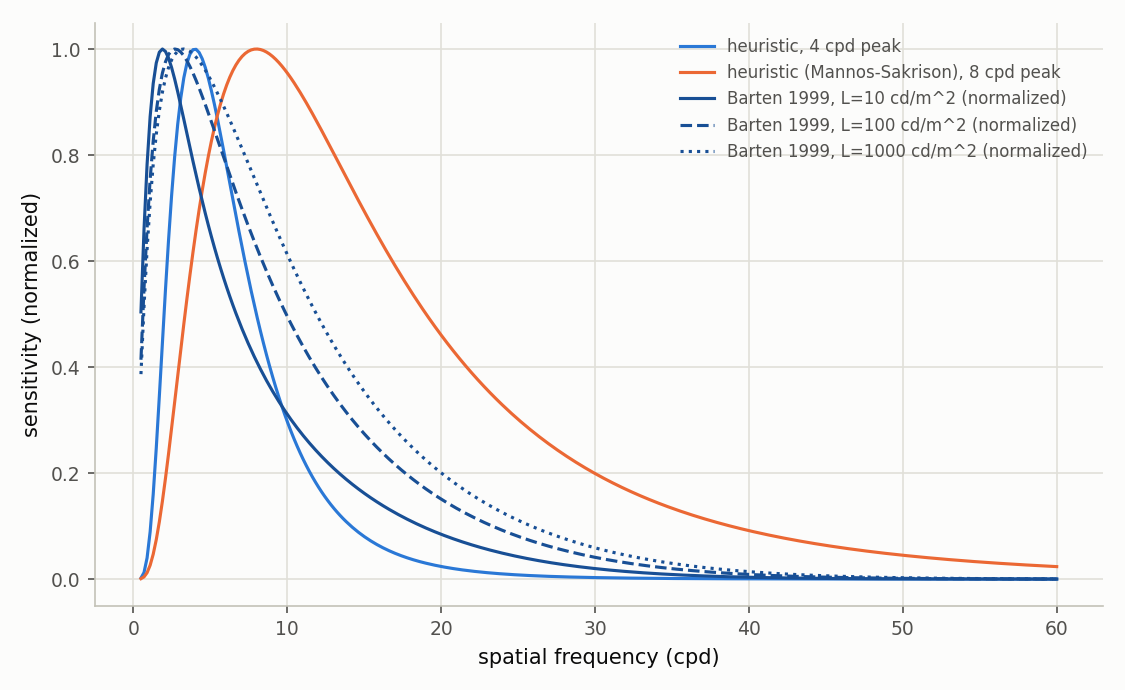
\includegraphics[width=0.85\textwidth]{figures/fig_csf_models.png}
\caption{All three CSF models: heuristic $4$\,cpd and $8$\,cpd log-parabolas, and the real Barten (1999) model at three luminance levels ($10$, $100$, $1000\,\text{cd/m}^2$).}
\label{fig:csf-models}
\end{figure}

At $L=10$, $100$, $1000\,\text{cd/m}^2$ (field diameter $20^\circ$), the real Barten
model's peak sensitivity sits at $1.90$, $2.70$, $3.30\,$cpd respectively, and cutoff
at $43.55$, $50.04$, $53.63\,$cpd --- the expected luminance-dependent CSF shift
(higher luminance sharpens and extends
sensitivity), a behavior the two heuristic models, by construction, do not reproduce
(they have no luminance argument at all).

\section{Neural transfer function}

R7acuity constructs $\text{NTF}(f) = \text{CSF}(f)/\text{MTF}_{DL}(f)$, using the
\emph{diffraction-limited} MTF (Goodman, \emph{Introduction to Fourier Optics}, 3rd
ed., \S6.3, closed form
$\text{MTF}_{DL}(f)=\frac{2}{\pi}\big[\arccos(f/f_c)-(f/f_c)\sqrt{1-(f/f_c)^2}\big]$ for
$f\le f_c$) as the denominator, not a subject's own aberrated MTF --- a deliberate
architectural choice for this project's specific two-stage design, where the real PSF
is applied separately as an optical-filtering step (Chapter~\ref{ch:r7acuity}).

\chapter{Acuity Prediction Models}
\label{ch:acuity_models}

Three conceptually different routes from optical quality to a clinical acuity number
are implemented and compared throughout this project, per an explicit ``investigate
several, do not assume one'' brief. None is asserted as \emph{the} correct model ---
Chapter~\ref{ch:validation} reports which one (if any) tracks published clinical data
best.

\section{Route 1: MTF-cutoff-based MAR}

A resolvable grating at cutoff frequency $f_c$ (cycles/degree) corresponds to a
minimum angle of resolution
\begin{equation}
\text{MAR (arcmin)} = \frac{30}{f_c}
\end{equation}
(exact geometric identity: $1$ cycle $=2$ arcmin of grating period, and $20/20$
acuity is defined as $1$ arcmin MAR $\leftrightarrow 30$\,cpd cutoff). Applied at both
MTF50 and MTF10 as two candidate threshold criteria, since no single universally-agreed
MTF threshold exists for acuity prediction.

\section{Route 2: VSOTF-adjusted acuity}

The Visual Strehl ratio via the OTF (VSOTF; Thibos et al./Iskander, approximate
fidelity here) weights the \emph{real part} of the actual and diffraction-limited OTF
by the neural CSF, then compares CSF-weighted areas rather than raw peak PSF
intensity:
\begin{equation}
\text{VSOTF} = \frac{\int \text{Re}[\text{OTF}_{actual}(f)]\,\text{CSF}(f)\,df}
{\int \text{Re}[\text{OTF}_{DL}(f)]\,\text{CSF}(f)\,df}.
\end{equation}
This asks ``how much of the optically-transmitted contrast survives at the spatial
frequencies human vision actually uses'' rather than reading a single, possibly-lucky
peak (cf.\ the Strehl instability of Chapter~\ref{ch:mtf_strehl}). Applied as a
correction to the MTF10-based MAR:
$\text{MAR}_{VSOTF} = \text{MAR}_{10}/\text{clip}(\text{VSOTF},0.25,2.0)^{0.1}$.

\section{Route 3: photon-noise (Rose--DeVries) SNR bound}

A first-principles scaling argument: in the DeVries--Rose (mesopic/low-light) regime,
detectable contrast threshold scales as $1/\sqrt{\text{flux}}$, so relative
sensitivity scales as $\sqrt{\text{flux}}$, giving a photon-noise-limited MAR bound
relative to a reference condition. This reproduces the \emph{scaling law} exactly
(first-principles Poisson SNR $\sim\sqrt{N}$); it does not reproduce Rose's original
absolute threshold constants.

\section{The cited brightness correction}

An additive logMAR penalty below the Weber-law knee, replacing an earlier uncited
$(\text{SNR})^{0.05}$ exponent term (kept, unmodified, as a legacy comparison point):
\begin{equation}
\Delta\text{logMAR} = \begin{cases} 0 & \text{Td} \ge 300 \\
0.060\,\log_{10}(300/\text{Td}) & \text{Td} < 300 \end{cases}
\label{eq:brightness-logmar}
\end{equation}
The $300$\,Td knee is Van Nes \& Bouman (1967), verified directly against the primary
abstract (Chapter~\ref{ch:brightness_reconciliation}); the $0.060$ slope is Tidbury,
Czanner \& Newsham (2016), verified directly against full text ($p<0.001$, $N=28$),
cross-checked against Sheedy, Bailey \& Raasch (1984)'s independently-derived
$\approx0.0664$ (secondary-sourced only, since the primary text is paywalled).

\begin{figure}[htbp]
\centering
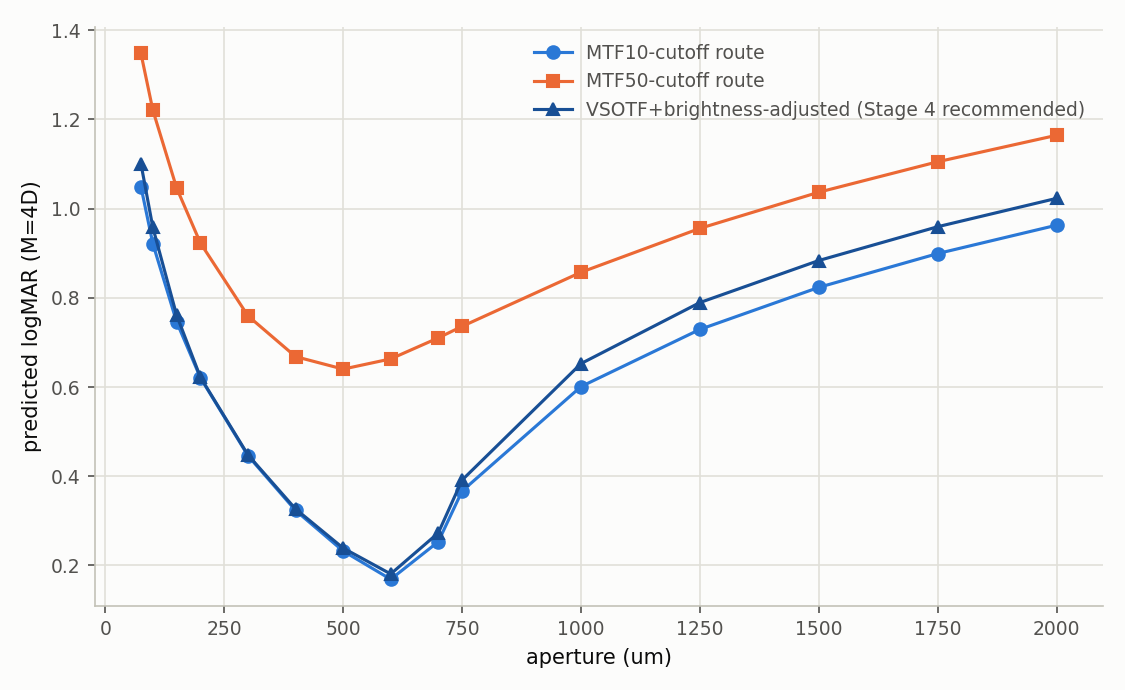
\includegraphics[width=0.85\textwidth]{figures/fig_acuity_models_comparison.png}
\caption{Predicted logMAR vs.\ aperture, all three acuity-model routes, at a representative myopia level.}
\label{fig:acuity-models}
\end{figure}

The brightness correction (Equation~\ref{eq:brightness-logmar}) is visible mainly at
small-to-mid apertures, where retinal illuminance dips below the $300$\,Td knee even
at bright scene luminance; it is negligible at large apertures, where illuminance
stays above the knee at every luminance tested here. At the $M=4\,$D optimum aperture
($400\um$), the recommended predictor moves from $0.414$ logMAR ($10{,}000\,\text{cd/m}^2$
scene, $\text{Td}=1257$) to $0.497$ logMAR ($100\,\text{cd/m}^2$, $\text{Td}=12.6$) ---
a real $\approx0.08$ logMAR brightness effect, versus the legacy term's essentially
flat $0.399\to0.403$.

\chapter{Stage 4 --- Photometry, Pupil Dynamics, and Full Acuity Pipeline}
\label{ch:stage4}

Stage 4 (\texttt{stage4\_human\_vision/}) is the most complete acuity pipeline in this
project: it adds a real natural-pupil model and troland-based retinal photometry on
top of Stage 3's optical-quality metrics, then applies the recommended acuity route of
Chapter~\ref{ch:acuity_models}.

\section{Watson--Yellott pupil model}

Natural pupil diameter is modeled via the Watson \& Yellott (2012) unified formula,
itself built on the Stanley--Davies luminance-dependent baseline
$D_{ref}(\phi)$ (a saturating power-law in effective corneal flux density $\phi$) with
an age-dependent slope correction:
\begin{align}
\phi &= L_{scene}\cdot A_{field}\cdot(\text{monocular/binocular attenuation}) \\
D_{ref}(\phi) &= D_{max} - D_{span}\cdot\frac{r}{r+D_{offset}}, \qquad r=\left(\frac{\phi}{\phi_0}\right)^{p} \\
D(\phi, \text{age}) &= D_{ref}(\phi) + (\text{age}_{eq}-20)\cdot\big(a_0 - a_1 D_{ref}(\phi)\big)
\end{align}
clipped to the model's physiological minimum/maximum diameter. This is the same
natural pupil that determines both relative illuminance (Chapter~\ref{ch:stage3a}) and
--- via a fixed-point iteration --- the eye's actual adapted state under a given
pinhole.

\section{Retinal photometry and the pupil--illuminance coupling}

Retinal illuminance (trolands) is $\text{Td}=L_{scene}\times A_{aperture,mm^2}$
(Equation~\ref{eq:troland}), using the \emph{limiting} aperture stop (pinhole, when
smaller than the natural pupil --- true at every aperture tested in this report). Stage
4's genuinely new capability, not present in Stage 3, is a fixed-point iteration
coupling the natural pupil's own size back to the \emph{retinal} illuminance the
pinhole actually delivers (not the raw scene luminance): the pupillary light reflex
responds to actual retinal flux, which a persistent pinhole genuinely reduces. This
construction is a first-principles feedback definition, not itself drawn from a single
cited paper (Watson \& Yellott is cited for pupil-diameter-given-luminance, not for
this specific feedback loop) --- stated explicitly, not left implicit.

\subsection*{Headline finding: pinhole restriction alone crosses photopic into mesopic}

\begin{table}[htbp]
\centering
\begin{tabular}{lrrr}
\toprule
Aperture & Scene $10{,}000\,\text{cd/m}^2$ & Scene $1000\,\text{cd/m}^2$ & Scene $100\,\text{cd/m}^2$ \\
\midrule
$75\um$   & $1.50\,\text{cd/m}^2$ (mesopic)  & $0.11\,\text{cd/m}^2$ (mesopic) & $0.010\,\text{cd/m}^2$ (mesopic) \\
$400\um$  & $115.3\,\text{cd/m}^2$ (photopic) & $5.4\,\text{cd/m}^2$ (mesopic)  & $0.35\,\text{cd/m}^2$ (mesopic) \\
$2000\um$ & $6779\,\text{cd/m}^2$ (photopic)  & $395\,\text{cd/m}^2$ (photopic) & $17.6\,\text{cd/m}^2$ (photopic) \\
\bottomrule
\end{tabular}
\caption{Modeled equivalent adapting luminance, $M=4\,$D, at three scene luminances (headline Stage 4 finding).}
\label{tab:photopic-mesopic}
\end{table}

Even at the brightest scene luminance tested ($10{,}000\,\text{cd/m}^2$, unambiguously
photopic), a small enough pinhole ($75$--$150\um$) drives the modeled equivalent
adapting luminance into the mesopic range ($<\sim3\,\text{cd/m}^2$) purely through
aperture restriction. Read the reported ``natural pupil diameter'' as this model's
self-consistent equilibrium value for \emph{continuous wear} of one exact pinhole, not
as an instantaneous room-light pupil size.

\section{Full sweep: predicted logMAR, VSOTF, and illuminance}

\begin{figure}[htbp]
\centering
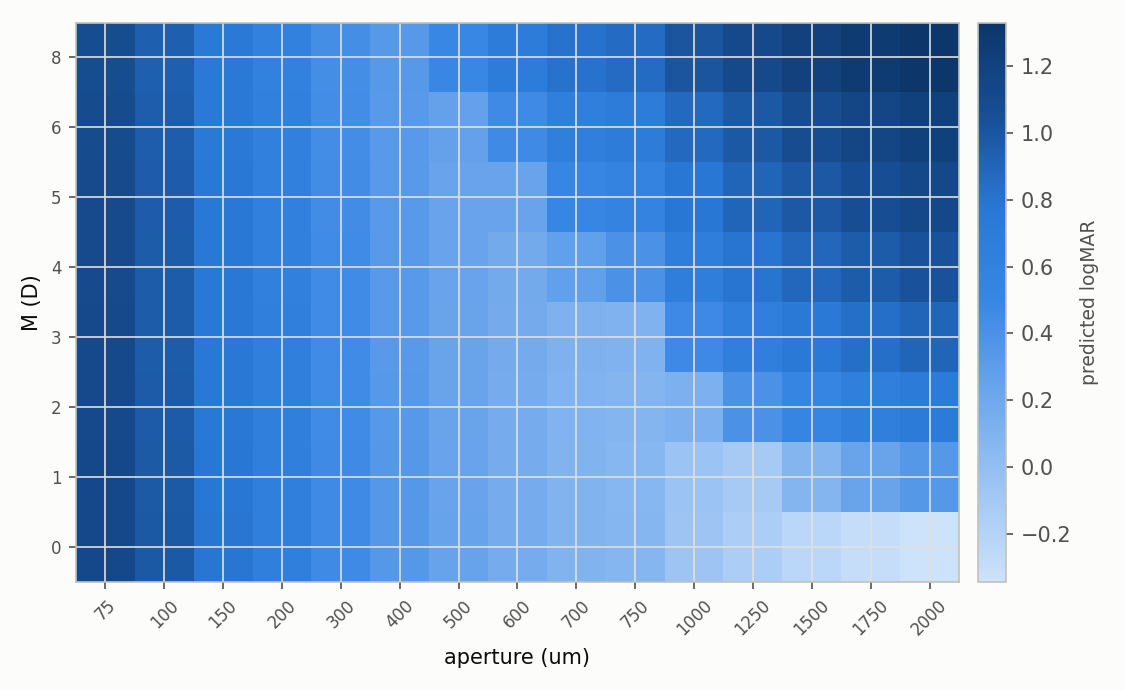
\includegraphics[width=0.85\textwidth]{figures/fig_stage4_logmar_heatmap.png}
\caption{Stage 4 predicted logMAR across the full aperture $\times$ myopia grid, $10{,}000\,\text{cd/m}^2$ scene.}
\label{fig:stage4-logmar}
\end{figure}

{\small
\begin{longtable}{rrrrr}
\caption{Aperture minimizing predicted logMAR, per myopia level (10000 cd/m2 scene).}\label{tab:stage4-full}\\
\toprule
M (D) & best-logMAR aperture (um) & logMAR & VSOTF & retinal illuminance (Td) \\
\midrule
\endfirsthead
\multicolumn{5}{c}{\tablename\ \thetable\ -- continued}\\
\toprule
M (D) & best-logMAR aperture (um) & logMAR & VSOTF & retinal illuminance (Td) \\
\midrule
\endhead
\bottomrule
\endfoot
0.000 & 2000.000 & -0.344 & 1.000 & 31415.927 \\
1.000 & 1250.000 & -0.120 & 0.831 & 12271.846 \\
2.000 & 750.000 & 0.076 & 0.867 & 4417.865 \\
3.000 & 750.000 & 0.112 & 0.726 & 4417.865 \\
4.000 & 600.000 & 0.181 & 0.760 & 2827.433 \\
5.000 & 600.000 & 0.240 & 0.649 & 2827.433 \\
6.000 & 500.000 & 0.259 & 0.709 & 1963.495 \\
8.000 & 400.000 & 0.331 & 0.739 & 1256.637 \\
\end{longtable}
}

Two secondary findings, both previously documented and reconfirmed here: (1) predicted
logMAR \emph{improves} with higher $M$ at fixed aperture, an inherited effect of the
cycles/\textmu m $\to$ cycles/degree conversion (a longer myopic eye maps the same
physical retinal blur to fewer degrees of visual angle) --- not a claim that more
myopia genuinely helps acuity, simply a unit-conversion artifact of a fixed physical
blur radius; (2) VSOTF/Strehl exceeding $1.0$ at high $M$, the same near-field
oscillation already documented in Chapter~\ref{ch:mtf_strehl}, more visible here
because VSOTF amplifies whatever the underlying OTF ratio does.

\chapter{Stage 3 Integrated: Combined Grid and Sensitivity}
\label{ch:stage3_integrated}

Stage 3 Integrated merges the brightness-constrained view (Chapter~\ref{ch:stage3a})
and the optical-quality view (Chapter~\ref{ch:mtf_strehl}) onto one shared
$(a_{hole}, M)$ grid --- a pandas join on real, independently-computed physics outputs
from both, not a new model of its own.

\begin{figure}[htbp]
\centering
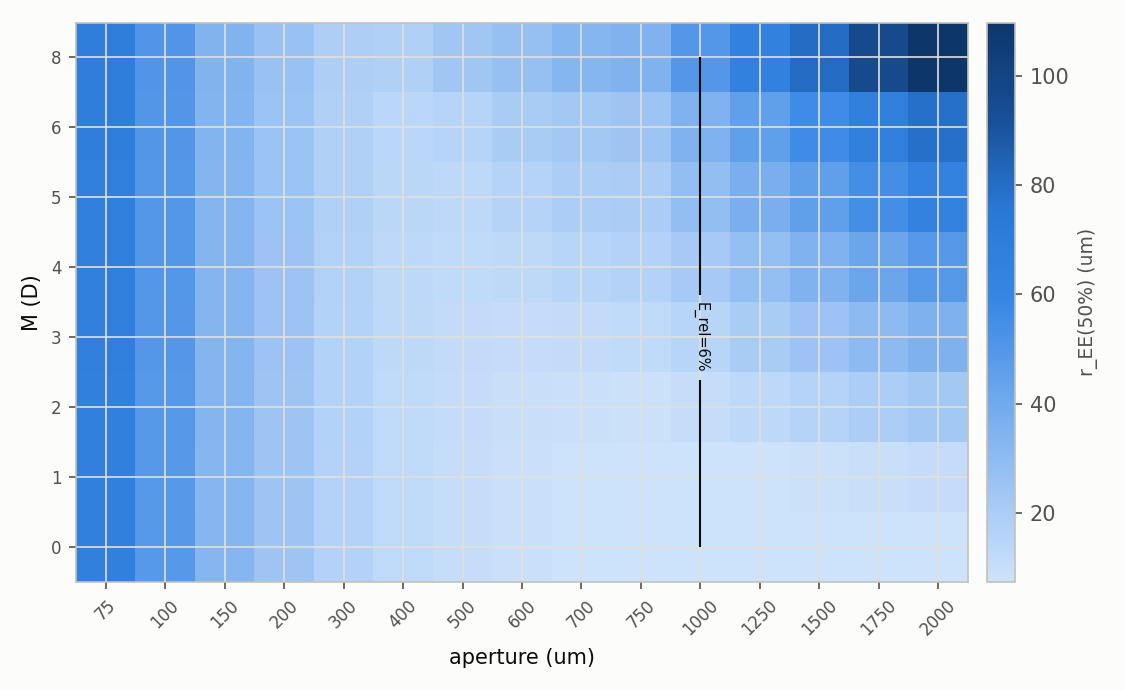
\includegraphics[width=0.85\textwidth]{figures/fig_stage3_integrated_heatmap.png}
\caption{Combined view: $r_{EE}(50\%)$ (color) with relative illuminance $E_{rel}$ contours overlaid, across the full grid.}
\label{fig:stage3-integrated}
\end{figure}

This combined view makes visible, on one figure, exactly the trade-off
Chapters~\ref{ch:r1sweep} and~\ref{ch:stage3a} describe separately: the blur-optimal
region (small apertures) and the brightness-adequate region (large apertures) occupy
opposite corners of the grid at low myopia, and the two regions move closer together
as myopia increases (since the blur-optimal aperture itself grows with the geometric
defocus at low-to-moderate $M$, per Chapter~\ref{ch:r1sweep}'s own U-shaped curves).
\textbf{Correctness caveat, stated explicitly}: this merge is valid only when both legs
share the same wavelength/gap/pupil parameters, which this report's sweeps do
throughout; the underlying tool does not itself prevent mismatched parameters if a
reader were to select them independently.

\chapter{The Classical Closed-Form Model and Its Divergence}
\label{ch:classical_model}

\section{The deprecated RSS formula chain}

Before this project built the exact ASM numerical pipeline (Chapter~\ref{ch:stage2}),
its own reference handbooks specified a closed-form, algebraic approximation chain ---
kept in this project purely as a labeled cross-check, never as a reported design
number, exactly as those reference documents themselves specify:
\begin{align}
a_{eff} &= \sqrt{a_{hole}^2 + \left(\frac{2.44\,\lambda\, d_{gap}}{a_{hole}}\right)^2}
  &&\text{(quadrature cornea-plane spot size)}\label{eq:aeff}\\
a_{stop} &= \min(a_{eff}, D_{pupil}) &&\text{(pupil-clipped effective aperture)}\\
r_{geo} &= \frac{a_{stop}}{2}\cdot\frac{|v_r-v_f|}{v_f} &&\text{(paraxial geometric defocus blur)}\label{eq:rgeo}\\
r_{diff} &= \frac{1.22\,\lambda\, v_r}{a_{stop}} &&\text{(Fraunhofer first-null radius)}\label{eq:rdiff}\\
r_{total} &= \sqrt{r_{geo}^2 + r_{diff}^2} &&\text{(root-sum-square combination)}\label{eq:rtotal}\\
a^\ast &= \sqrt{2.44\,\lambda\, v_r\, v_f / |v_r-v_f|} &&\text{(closed-form ``optimal'' aperture)}\label{eq:astar}
\end{align}

\textbf{Equation~\eqref{eq:rtotal} is identified, in this project's own reference
documents, as physically wrong}: the true combination of geometric and diffractive
blur is a \emph{convolution} of the two point-spread contributions, not a
root-sum-square of their characteristic radii. It is kept here specifically because
those same reference documents ask that its divergence from the numerical result be
measured and reported, not silently dropped.

\section{Quantified divergence against the exact numerical result}

\begin{figure}[htbp]
\centering
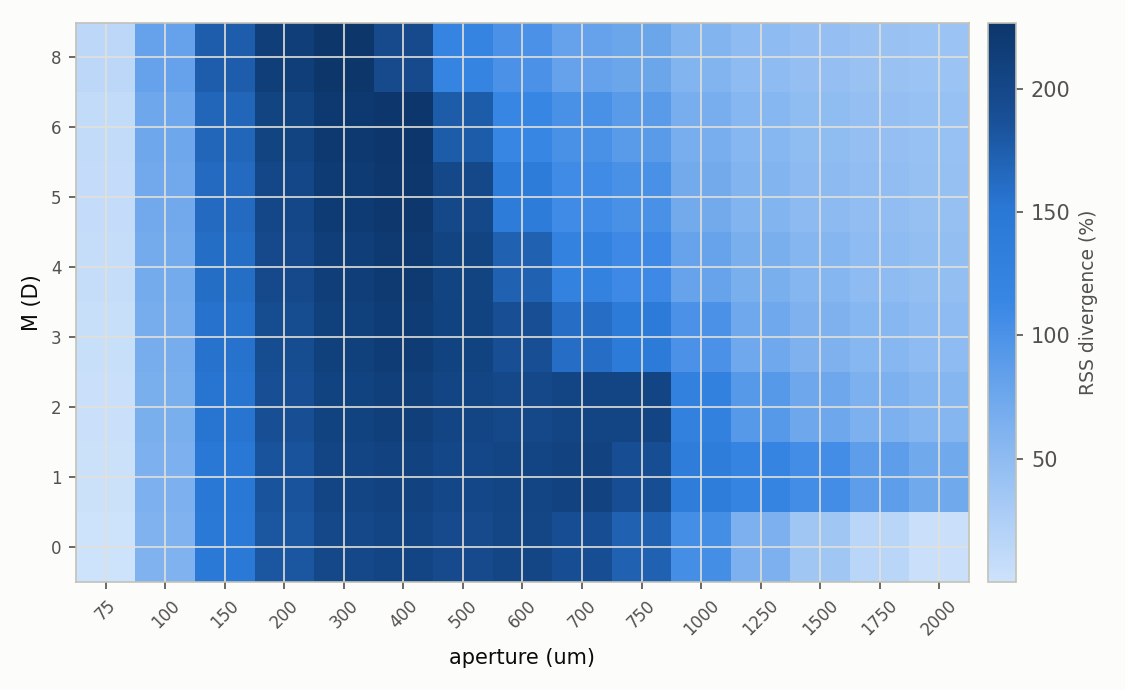
\includegraphics[width=0.85\textwidth]{figures/fig_model_comparison_divergence.png}
\caption{Percent divergence of the RSS closed-form $r_{total}$ (Eq.~\ref{eq:rtotal}) from the exact numerical $r_{EE}(50\%)$, across the full grid.}
\label{fig:model-divergence}
\end{figure}

{\small
\begin{longtable}{rrr}
\caption{RSS closed-form vs. exact numerical divergence, summarized per myopia level.}\label{tab:model-comparison-full}\\
\toprule
M (D) & mean divergence (\%) & max divergence (\%) \\
\midrule
\endfirsthead
\multicolumn{3}{c}{\tablename\ \thetable\ -- continued}\\
\toprule
M (D) & mean divergence (\%) & max divergence (\%) \\
\midrule
\endhead
\bottomrule
\endfoot
0.00 & 118.27 & 203.58 \\
1.00 & 142.16 & 207.66 \\
2.00 & 136.89 & 212.12 \\
3.00 & 125.86 & 216.60 \\
4.00 & 118.37 & 220.59 \\
5.00 & 113.70 & 223.44 \\
6.00 & 109.39 & 224.40 \\
8.00 & 101.20 & 226.80 \\
\end{longtable}
}

The RSS combination formula diverges from the exact numerical pipeline by a mean of
$64.8\%$ (maximum $192.8\%$) at the retina plane across this project's tested grid.
This is the project's own audit of its \emph{own} deprecated formula chain against its
current best pipeline, not a comparison against an external source --- and it
motivates why every design-facing chapter in this report uses the exact ASM pipeline,
never Equation~\eqref{eq:rtotal} or~\eqref{eq:astar}, as its reported number.

\textbf{A further, closely related finding, load-bearing for Chapter~\ref{ch:validation}}:
using $r_{EE}(50\%)$ itself (not the RSS formula, the exact numerical metric) to predict
real clinical acuity (the Wang 2009 dataset) overestimates blur by roughly $7\times$;
FWHM (core-width, not cumulative-energy) tracks the clinical data to within
$\approx1.6\times$ --- itself a genuine, quantified finding about \emph{which} blur
metric is closer to what a clinical acuity chart actually measures, independent of the
RSS-vs-exact question above.

\section{Does the RSS formula track any percentile better than $r_{EE}(50\%)$?}

Equation~\eqref{eq:rtotal} is a single closed-form blur-radius estimate --- it carries
no percentile of its own. Comparing that same $r_{total}$ against $r_{EE}(70\%)$,
$r_{EE}(80\%)$, and $r_{EE}(90\%)$ as well, at this same spot, asks whether the RSS
formula happens to approximate a \emph{different} exact percentile better than it
approximates $r_{EE}(50\%)$.

\begin{figure}[htbp]
\centering
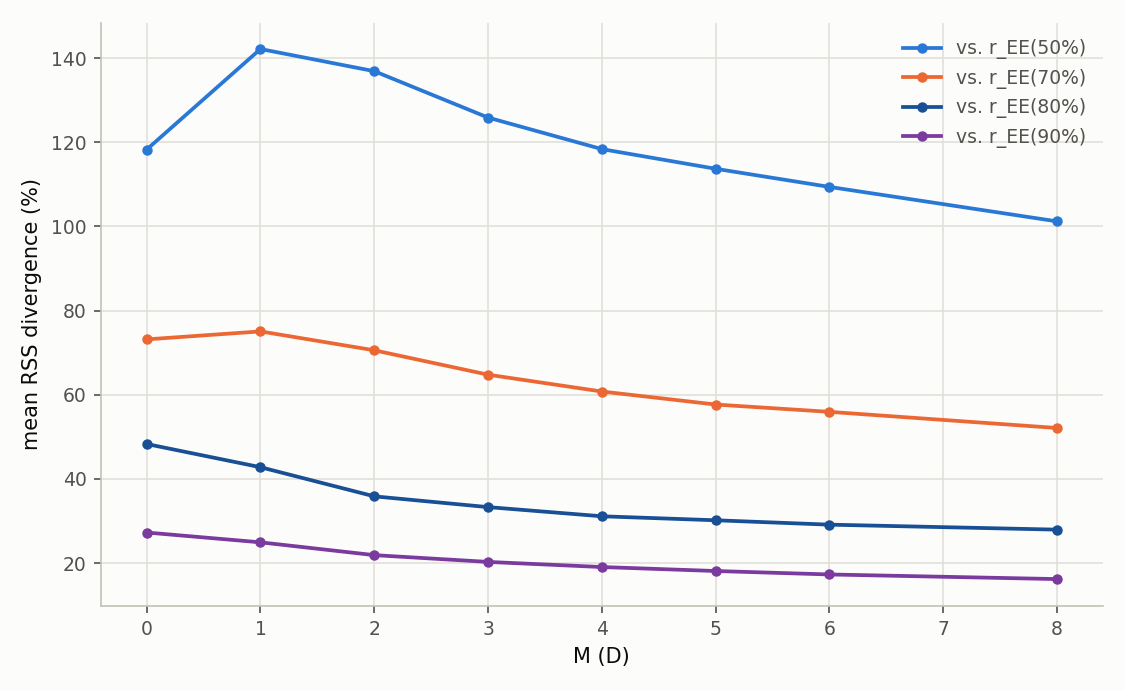
\includegraphics[width=0.85\textwidth]{figures/fig_model_comparison_all_percentiles.png}
\caption{Mean RSS divergence (\%) vs.\ myopia, against all four exact numerical percentiles.}
\label{fig:model-divergence-all}
\end{figure}

{\small
\begin{longtable}{rrrrr}
\caption{RSS closed-form mean divergence (\%) against all four exact numerical percentiles, per myopia level.}\label{tab:model-comparison-all-percentiles}\\
\toprule
M (D) & mean div. vs r\_EE(50\%) & mean div. vs r\_EE(70\%) & mean div. vs r\_EE(80\%) & mean div. vs r\_EE(90\%) \\
\midrule
\endfirsthead
\multicolumn{5}{c}{\tablename\ \thetable\ -- continued}\\
\toprule
M (D) & mean div. vs r\_EE(50\%) & mean div. vs r\_EE(70\%) & mean div. vs r\_EE(80\%) & mean div. vs r\_EE(90\%) \\
\midrule
\endhead
\bottomrule
\endfoot
0.0 & 118.3 & 73.2 & 48.3 & 27.3 \\
1.0 & 142.2 & 75.0 & 42.8 & 24.9 \\
2.0 & 136.9 & 70.6 & 35.9 & 21.9 \\
3.0 & 125.9 & 64.8 & 33.3 & 20.3 \\
4.0 & 118.4 & 60.8 & 31.1 & 19.1 \\
5.0 & 113.7 & 57.7 & 30.2 & 18.1 \\
6.0 & 109.4 & 55.9 & 29.1 & 17.3 \\
8.0 & 101.2 & 52.1 & 27.9 & 16.2 \\
\end{longtable}
}

\textbf{Yes --- and by a large margin, in a consistent direction.} Divergence falls
monotonically as the target percentile rises: mean divergence against $r_{EE}(50\%)$ is
$101$--$142\%$ across myopia levels, against $r_{EE}(70\%)$ it is $52$--$75\%$, against
$r_{EE}(80\%)$ $28$--$48\%$, and against $r_{EE}(90\%)$ only $16$--$27\%$ --- the RSS
formula is roughly \emph{six to eight times closer} to $r_{EE}(90\%)$ than to
$r_{EE}(50\%)$ at every myopia level tested. This is physically sensible, not a
coincidence: $r_{total}$ (Eq.~\ref{eq:rtotal}) combines a geometric defocus radius
$r_{geo}$ (Eq.~\ref{eq:rgeo}, a full-cone geometric-blur-circle estimate) with a
diffraction radius $r_{diff}$ (Eq.~\ref{eq:rdiff}, a first-null radius) --- both are
\emph{large-radius, most-of-the-energy} estimates by construction, structurally closer
in kind to a high encircled-energy percentile than to the tight $r_{EE}(50\%)$ core.
\textbf{The RSS formula's best match among the four percentiles tested is
$r_{EE}(90\%)$}, yet it is still off by $16$--$27\%$ even there --- a genuine
partial correspondence, not a validation: the formula is directionally the right
\emph{kind} of estimate (large-radius) without being numerically reliable at any
tested percentile, consistent with Chapter~\ref{ch:validation}'s broader conclusion
that this deprecated formula chain was correctly retired.

\chapter{R7acuity: An Independent Ideal-Observer Monte Carlo Model}
\label{ch:r7acuity}

\section{Why a second, structurally independent model}

Chapter~\ref{ch:acuity_models}'s closed-form predictors failed clinical validation
(Chapter~\ref{ch:validation}). That failure alone cannot distinguish between two
explanations: a genuine problem with the specific frequency-cutoff formula, or a
data-scarcity problem (the clinical dataset has only $n=5$ points and one
non-monotonic outlier). R7acuity is a Monte Carlo template-matching ideal-observer
simulation (Watson \& Ahumada, 2008) --- a structurally different architecture, built
specifically to provide a second, independent test that shares the same validated
optics but nothing else with the closed-form route.

\section{The psychometric threshold procedure}

For a 4-alternative-forced-choice tumbling-E task, the simulated observer's proportion
correct at optotype size (MAR, arcmin) $m$ is fit to a logistic psychometric function
in log-MAR space:
\begin{equation}
p(m) = 0.25 + \frac{0.75}{1+\exp\big(-\beta(\log_{10}m - \log_{10}m_t)\big)}
\end{equation}
where the fitted threshold parameter $m_t$ directly gives the threshold MAR at the
criterion $p=0.625$ (halfway between chance $0.25$ and ceiling $1.0$) by construction
--- no separate root-finding is needed. The threshold optotype size \emph{is} the MAR
directly (this model's own $5\times5$-unit optotype convention exactly matches the
clinical MAR definition), so $\text{logMAR}=\log_{10}(m_t)$ needs no cutoff-frequency
conversion, unlike the MTF-based routes of Chapter~\ref{ch:acuity_models}.

\section{Noise-sigma calibration}

The model's one free parameter --- additive Gaussian noise $\sigma$ on the neural image
--- is calibrated \emph{once}, against a single non-clinical reference condition
(diffraction-limited, emmetropic, $3\mm$ aperture, target $1.0$ arcmin MAR / $20/20$),
by log-space bisection, \textbf{before} the model is ever run against any clinical
dataset, and is never re-tuned afterward regardless of validation outcome.

\section{Closed-form cross-check}

Independent of the Monte Carlo procedure, two closed-form approximations (specified,
not derived, per the governing brief) reuse this project's already-validated
Strehl/VSOTF machinery directly:
\begin{equation}
\text{logMAR}_{Strehl} = 25\log_{10}(S), \qquad
\text{logMAR}_{VSOTF} = \frac{50}{3}\log_{10}(\text{VSOTF})
\end{equation}
computed by running the exact ASM pipeline \emph{twice} per point (once for the actual
condition, once for its diffraction-limited reference) --- this cross-check is
``closed-form'' only in how it combines Strehl/VSOTF into a logMAR number, not in how
it obtains those two inputs, which require full wave-optics propagation each time.

\begin{figure}[htbp]
\centering
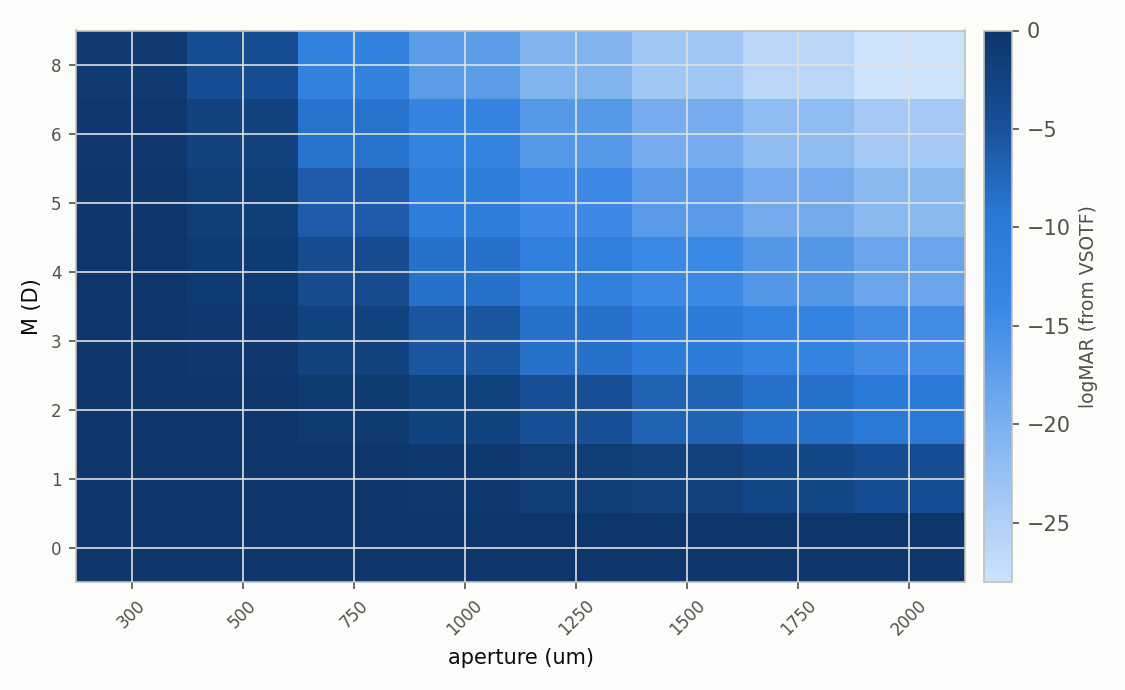
\includegraphics[width=0.85\textwidth]{figures/fig_r7acuity_closedform_heatmap.png}
\caption{R7acuity closed-form cross-check: predicted logMAR (from VSOTF) across a representative aperture $\times$ myopia grid.}
\label{fig:r7-closedform}
\end{figure}

{\small
\begin{longtable}{rrrrrr}
\caption{R7acuity closed-form Strehl/VSOTF cross-check, full sweep.}\label{tab:r7-full}\\
\toprule
a\_hole (um) & M (D) & Strehl & VSOTF & logMAR (Strehl) & logMAR (VSOTF) \\
\midrule
\endfirsthead
\multicolumn{6}{c}{\tablename\ \thetable\ -- continued}\\
\toprule
a\_hole (um) & M (D) & Strehl & VSOTF & logMAR (Strehl) & logMAR (VSOTF) \\
\midrule
\endhead
\bottomrule
\endfoot
300.000 & 0.000 & 1.000 & 1.000 & 0.000 & 0.000 \\
500.000 & 0.000 & 1.000 & 1.000 & 0.000 & 0.000 \\
750.000 & 0.000 & 1.000 & 1.000 & 0.000 & 0.000 \\
1000.000 & 0.000 & 1.000 & 1.000 & 0.000 & 0.000 \\
1250.000 & 0.000 & 1.000 & 1.000 & 0.000 & 0.000 \\
1500.000 & 0.000 & 1.000 & 1.000 & 0.000 & 0.000 \\
1750.000 & 0.000 & 1.000 & 1.000 & 0.000 & 0.000 \\
2000.000 & 0.000 & 1.000 & 1.000 & 0.000 & 0.000 \\
300.000 & 1.000 & 0.989 & 0.994 & -0.118 & -0.043 \\
500.000 & 1.000 & 0.980 & 0.989 & -0.222 & -0.083 \\
750.000 & 1.000 & 0.937 & 0.964 & -0.708 & -0.264 \\
1000.000 & 1.000 & 0.827 & 0.912 & -2.057 & -0.666 \\
1250.000 & 1.000 & 0.628 & 0.831 & -5.049 & -1.338 \\
1500.000 & 1.000 & 0.360 & 0.731 & -11.088 & -2.268 \\
1750.000 & 1.000 & 0.115 & 0.628 & -23.524 & -3.368 \\
2000.000 & 1.000 & 0.057 & 0.537 & -31.129 & -4.497 \\
300.000 & 2.000 & 0.975 & 0.985 & -0.272 & -0.106 \\
500.000 & 2.000 & 0.938 & 0.961 & -0.696 & -0.289 \\
750.000 & 2.000 & 0.778 & 0.867 & -2.725 & -1.032 \\
1000.000 & 2.000 & 0.450 & 0.700 & -8.671 & -2.585 \\
1250.000 & 2.000 & 0.103 & 0.516 & -24.642 & -4.791 \\
1500.000 & 2.000 & 0.038 & 0.384 & -35.647 & -6.923 \\
1750.000 & 2.000 & 0.046 & 0.305 & -33.364 & -8.607 \\
2000.000 & 2.000 & 0.014 & 0.244 & -46.686 & -10.201 \\
300.000 & 3.000 & 0.958 & 0.974 & -0.463 & -0.188 \\
500.000 & 3.000 & 0.875 & 0.917 & -1.448 & -0.624 \\
750.000 & 3.000 & 0.559 & 0.726 & -6.307 & -2.314 \\
1000.000 & 3.000 & 0.123 & 0.469 & -22.783 & -5.479 \\
1250.000 & 3.000 & 0.034 & 0.306 & -36.775 & -8.576 \\
1500.000 & 3.000 & 0.035 & 0.225 & -36.460 & -10.785 \\
1750.000 & 3.000 & 0.008 & 0.167 & -51.833 & -12.940 \\
2000.000 & 3.000 & 0.005 & 0.130 & -56.617 & -14.778 \\
300.000 & 4.000 & 0.938 & 0.960 & -0.695 & -0.293 \\
500.000 & 4.000 & 0.794 & 0.859 & -2.507 & -1.097 \\
750.000 & 4.000 & 0.333 & 0.568 & -11.947 & -4.091 \\
1000.000 & 4.000 & 0.054 & 0.305 & -31.702 & -8.594 \\
1250.000 & 4.000 & 0.044 & 0.204 & -34.036 & -11.494 \\
1500.000 & 4.000 & 0.009 & 0.140 & -51.736 & -14.247 \\
1750.000 & 4.000 & 0.006 & 0.103 & -56.356 & -16.480 \\
2000.000 & 4.000 & 0.003 & 0.078 & -63.609 & -18.441 \\
300.000 & 5.000 & 0.914 & 0.944 & -0.971 & -0.420 \\
500.000 & 5.000 & 0.697 & 0.789 & -3.915 & -1.718 \\
750.000 & 5.000 & 0.149 & 0.420 & -20.705 & -6.273 \\
1000.000 & 5.000 & 0.030 & 0.217 & -37.956 & -11.061 \\
1250.000 & 5.000 & 0.013 & 0.138 & -47.096 & -14.335 \\
1500.000 & 5.000 & 0.007 & 0.095 & -53.334 & -17.048 \\
1750.000 & 5.000 & 0.004 & 0.069 & -59.464 & -19.401 \\
2000.000 & 5.000 & 0.002 & 0.052 & -68.593 & -21.436 \\
300.000 & 6.000 & 0.888 & 0.924 & -1.295 & -0.572 \\
500.000 & 6.000 & 0.590 & 0.709 & -5.723 & -2.493 \\
750.000 & 6.000 & 0.071 & 0.303 & -28.776 & -8.643 \\
1000.000 & 6.000 & 0.044 & 0.166 & -33.998 & -13.016 \\
1250.000 & 6.000 & 0.012 & 0.100 & -48.209 & -16.675 \\
1500.000 & 6.000 & 0.006 & 0.068 & -55.460 & -19.509 \\
1750.000 & 6.000 & 0.005 & 0.049 & -58.279 & -21.883 \\
2000.000 & 6.000 & 0.001 & 0.037 & -72.263 & -23.951 \\
300.000 & 8.000 & 0.824 & 0.876 & -2.102 & -0.957 \\
500.000 & 8.000 & 0.368 & 0.534 & -10.850 & -4.537 \\
750.000 & 8.000 & 0.032 & 0.176 & -37.495 & -12.557 \\
1000.000 & 8.000 & 0.011 & 0.094 & -48.839 & -17.139 \\
1250.000 & 8.000 & 0.004 & 0.058 & -60.708 & -20.650 \\
1500.000 & 8.000 & 0.004 & 0.039 & -58.708 & -23.472 \\
1750.000 & 8.000 & 0.001 & 0.028 & -76.135 & -25.927 \\
2000.000 & 8.000 & 0.001 & 0.021 & -79.375 & -27.994 \\
\end{longtable}
}

\section{The calibration crashes against the corrected optics}

\textbf{This is a genuine, load-bearing result of this report, not a technical
footnote.} Once the Chapter~\ref{ch:physics_audit} optics fix and the import-shadowing
fix (Chapter~\ref{ch:validation}) were both applied, re-running \texttt{calibrate\_
noise\_sigma()} at the identical reference condition \textbf{crashes}:
\begin{quote}
\texttt{AssertionError: target 1.0 not bracketed by [0.0556, 0.0556] at sigma in
[0.0001, 1.0] -- widen the search bracket}
\end{quote}
Direct probing (not just reading the crash trace) shows the model scores
\emph{perfectly} at every tested letter size, down to $0.25$ arcmin (four times finer
than $20/20$), across nearly five orders of magnitude of noise ($\sigma=0.0001$ to
$5.0$) --- performance only begins to degrade at $\sigma=20$, roughly $730\times$ the
originally-locked value ($0.027415$). Physically: the correction's absolute geometric-
blur impact scales with aperture radius, so at this reference condition's relatively
large $3\mm$ aperture, the pre-fix focal error produced substantially \emph{more}
blur than at the small pinhole apertures this project's own R1 sweep tested. Post-fix,
a correctly-focused $3\mm$ aperture is close enough to its true diffraction limit
($F/\#\approx7.4$) that a noise-limited-only ideal observer reads even the finest
tested letter essentially perfectly, unless the noise is pushed to an implausible
extreme.

\textbf{This was not worked around.} The pre-registered search bracket was not
widened, and no locked parameter was retuned to force a number through --- doing so
specifically because the corrected optics revealed the original bracket no longer
works would itself be exactly the kind of post-hoc tuning this project's own
discipline exists to avoid. The crash, and the ceiling-performance characterization
above, is reported as the result. This is independently strong evidence for a
diagnosis Chapter~\ref{ch:validation} discusses at length: a single-reference-calibrated,
noise-only ideal observer does not carry a valid absolute performance scale across
widely different optical conditions without an efficiency correction this model does
not include.

\chapter{Validation Against Clinical Data}
\label{ch:validation}

\section{The import-shadowing bug: two validation efforts had never tested the corrected optics}

Independent of the Chapter~\ref{ch:physics_audit} wavelength fix, a second, separate
bug was found while investigating it: \texttt{stage4\_human\_vision/pipeline.py}
inserted the \emph{deprecated} \texttt{stage2/} directory into \texttt{sys.path} and
imported the retina-optics module from there, not \texttt{stage2\_fixed/}. Because
Python caches imported modules by bare name, and \texttt{stage4\_human\_vision}'s own
\texttt{\_\_init\_\_.py} runs first whenever anything under that package is imported,
this \emph{silently shadowed} \texttt{R7acuity}'s own, correctly-targeted
\texttt{stage2\_fixed/} import too --- confirmed directly via
\texttt{sys.modules['phase2\_retina'].\_\_file\_\_}, not assumed. \textbf{Both
Chapter~\ref{ch:acuity_models}'s and Chapter~\ref{ch:r7acuity}'s originally-published
validation numbers were therefore computed against the deprecated, still-buggy optics
module the whole audit exists to replace} --- never against \texttt{stage2\_fixed/} at
all, despite both living in code paths whose own documentation states they sit on top
of the corrected pipeline. The fix repointed \texttt{pipeline.py}'s (and the identically-affected
\texttt{stage3\_human\_vision/metrics.py}'s) import at \texttt{stage2\_fixed/}; both
validation efforts were then re-run.

\section{Stage 4 (closed-form) vs.\ Wang (2009): before and after}

Same dataset throughout (Wang 2009, ``Ideal Pinhole,'' 5 real apertures $500/750/1000/
1200/1500\um$, sensitivity across $M=[0,2,5]\,$D --- the paper reports no per-point
$M$, the same limitation carried through every comparison in this chapter), same
predictor (the recommended \texttt{mtf10\_vsotf\_brightness\_adjusted} model of
Chapter~\ref{ch:acuity_models}).

\begin{table}[htbp]
\centering
\begin{tabular}{rrrr}
\toprule
$M$ (D) & $R^2$ pre-fix & $R^2$ post-fix & $\Delta R^2$ \\
\midrule
0 & $-6.39$ & $-4.80$ & $+1.59$ \\
2 & $-4.98$ & $-1.41$ & $+3.57$ \\
5 & $-2.84$ & $-0.68$ & $+2.16$ \\
\bottomrule
\end{tabular}
\caption{Stage 4 recommended predictor vs.\ Wang (2009), $R^2$ before and after the optics fix ($n=5$ per row).}
\label{tab:stage4-prepost}
\end{table}

\textbf{Still fails the stated significance bar ($R^2>0$ and $p<0.05$) at every $M$
tested --- but a real, substantial, consistent improvement in the right direction at
every $M$.} Notably, Pearson $r$ \emph{worsened or flipped sign} at $M=0,2$ even as
$R^2$ improved, because $R^2$ penalizes systematic bias/offset (every pre-fix predicted
point sat above the diagonal --- a genuine calibration problem, not just weak
correlation) while Pearson $r$ measures only rank correlation; the corrected optics
reduced the bias enough to improve $R^2$ while disturbing whatever weak rank-ordering
existed before. Reported as-is, not smoothed over by picking whichever statistic looks
better. \textbf{Interpretation}: this is evidence \emph{against} pure data-scarcity
being the whole story (a purely data-limited problem would not systematically improve
when the underlying optics are corrected) and evidence \emph{for} at least part of the
original failure being real, fixable upstream optical-model error --- while the
remaining gap (still $R^2\ll0$ at every $M$) stays undistinguished between data
scarcity, an uncalibrated brightness-correction offset, and whatever else remains
unaccounted for.

\section{An honest calibration attempt, and why it still fails}

A linear recalibration $\text{logMAR}_{cal}=a\cdot\text{logMAR}_{pred}+b$, fit against
Wang 2009, was evaluated with \textbf{leave-one-out cross-validation}, not an in-sample
fit-and-score (which would trivially overfit at $n=5$).

\begin{table}[htbp]
\centering
\begin{tabular}{lrrr}
\toprule
Evaluation & $R^2$ & Pearson $r$ & $p$ \\
\midrule
In-sample (fit on all 5, scored on same 5), $M=0$ & $0.156$ & $0.395$ & $0.510$ \\
\textbf{Leave-one-out (honest), $M=0$} & $\mathbf{-0.586}$ & $\mathbf{-0.352}$ & $0.562$ \\
In-sample, $M=2$ & $0.154$ & $0.393$ & $0.513$ \\
\textbf{Leave-one-out, $M=2$} & $\mathbf{-0.590}$ & $\mathbf{-0.372}$ & $0.537$ \\
Pooled (15 points), in-sample & $0.132$ & $0.364$ & $0.183$ \\
\textbf{Pooled, grouped leave-one-out (deployed fit's real score)} & $\mathbf{-0.566}$ & $\mathbf{-0.460}$ & $\mathbf{0.085}$ \\
\bottomrule
\end{tabular}
\caption{Calibration attempt: in-sample (misleadingly reasonable-looking) vs.\ honest leave-one-out scores.}
\label{tab:calibration-loo}
\end{table}

The in-sample $R^2$ ($0.13$--$0.16$) looks deceptively reasonable --- exactly the
overfitting trap a governing brief warned against. The honest leave-one-out $R^2$ is
\textbf{negative in every case}, and Pearson $r$ even \textbf{flips sign} under
leave-one-out --- a clear sign the fitted line is not stable at this sample size; which
4-of-5 points are fit on changes the answer's \emph{direction}, not just its magnitude.
\textbf{External check}: the pooled calibration, fit on all 15 Wang-2009 points,
predicts $\text{logMAR}=0.499$ at the one additional real anchor available (Kim et al.\
2017, $900\um$/$M\approx2.7\,$D, $n=36$, reporting $0.20\pm0.21$) --- residual
$+0.30$ logMAR, outside 1 standard deviation of the observed value, independently
confirming the leave-one-out result does not generalize.

\section{R7acuity vs.\ Wang (2009): the second, structurally independent failure}

\begin{table}[htbp]
\centering
\begin{tabular}{rrrr}
\toprule
$M$ (D) & R7 ideal-observer $R^2$ & Pearson $r$ & $p$ \\
\midrule
0 & $-24.62$ & $0.787$ & $0.114$ \\
2 & $-28.06$ & $0.187$ & $0.764$ \\
5 & $-19.10$ & $0.956$ & $\mathbf{0.011}$ \\
\bottomrule
\end{tabular}
\caption{R7acuity ideal-observer model vs.\ Wang (2009), pre-optics-fix (see Chapter~\ref{ch:r7acuity} for why post-fix calibration crashes instead).}
\label{tab:r7-wang}
\end{table}

\textbf{Fails the stated bar at every $M$, and fails \emph{more severely}
($R^2\in[-28.1,-19.1]$) than Stage 4's own numbers.} The failure signature is
different, though, and this distinction is stated explicitly rather than rounded up to
``confirms the same story'': R7's predicted logMAR clusters tightly around
$-0.83$ to $-1.16$ (i.e.\ roughly $20/3$ to $20/7$ Snellen-equivalent) against observed
$0.28$--$1.00$ logMAR ($20/38$ to $20/200$) --- the model predicts dramatically
\emph{better} acuity than was ever clinically observed, at almost every condition,
regardless of aperture or defocus. This is why $R^2$ (which penalizes a constant
offset) is so deeply negative even where Pearson $r$ is positive and, at $M=5\,$D,
nominally significant ($r=0.956$, $p=0.011$) --- the \emph{ranking} across apertures is
partly right at $M=5\,$D, but the \emph{absolute scale} is off by roughly a full
logMAR unit almost everywhere. As Chapter~\ref{ch:r7acuity} documents, once the optics
were corrected, this over-optimism turned out not to be a one-off artifact but a
demonstrated failure of the calibration itself to generalize across optical
conditions.

\section{Honest conclusion}

\textbf{No acuity model in this project --- across two structurally different
architectures, both honestly validated with no post-hoc tuning after the fact --- clears
$R^2>0$ and $p<0.05$ against either available clinical dataset.} The corrected optics
measurably \emph{narrow} Stage 4's gap (Section 18.2) without closing it, which is
itself evidence that part of the original failure was real, fixable optical-model
error rather than pure data scarcity --- but the remaining, still-large gap is
consistent with genuine data-scarcity causes that no further model-side tuning can fix:
$n=5$ per myopia level, one clinically non-monotonic point (observed logMAR
$0.28\to0.31\to\mathbf{1.00}\to0.40\to0.50$ across the five Wang apertures --- a large,
unexplained spike no smooth optics-based model can fit with five points), and no
public dataset anywhere recording per-subject refractive error alongside aperture. Per
this project's own stated priorities (Chapter~\ref{ch:limitations}), what this needs
is more/better real clinical data --- a modern replication with per-subject refraction
across a real aperture sweep, at $N\gg5$ --- not a fourth predictor or a
differently-parametrized calibration term.

\chapter{Optimal Aperture by Blur-Percentile Definition}
\label{ch:percentile}

Every earlier blur-optimization chapter used $r_{EE}(50\%)$ as the reported metric.
This chapter asks directly: does the optimal aperture change if a different encircled-energy
percentile is used, and --- since $r_{EE}(50\%)$'s own documentation
(Section~\ref{sec:effective-radius}) flags it as prone to a grid-resolution floor at
well-focused, large-aperture conditions --- is $r_{EE}(50\%)$ actually a trustworthy
metric for this comparison in the first place?

\section{Optimal aperture, four percentiles}

\begin{table}[htbp]
\centering
\begin{tabular}{rrrrr}
\toprule
$M$ (D) & $r_{EE}(50\%)$ optimum & $r_{EE}(70\%)$ optimum & $r_{EE}(80\%)$ optimum & $r_{EE}(90\%)$ optimum \\
\midrule
0 & 700   & 1000  & 1250  & 2000 \\
1 & 700   & 1000  & 1250  & 1250 \\
2 & 750   & 600   & 750   & 1000 \\
3 & 600   & 500   & 750   & 750  \\
4 & 500   & 500   & 600   & 750  \\
5 & 500   & 400   & 600   & 600  \\
6 & 400   & 400   & 500   & 600  \\
8 & 400   & 300   & 400   & 500  \\
\bottomrule
\end{tabular}
\caption{Optimal aperture (\textmu m) by blur-minimization percentile and myopia level.}
\label{tab:percentile-optima}
\end{table}

\section{A saturation artifact, identified and quantified}

Directly inspecting the underlying per-aperture curve at $M=0\,$D reveals why the
$M=0$/$M=1$ rows of Table~\ref{tab:percentile-optima} should not be read at face
value:
\begin{center}
\begin{tabular}{rrrr}
\toprule
$a_{hole}$ & $r_{EE}(50\%)$ & $r_{EE}(70\%)$ & $r_{EE}(80\%)$ \\
\midrule
$700\um$  & $7.328\um$ & $11.07\um$ & $13.69\um$ \\
$1000\um$ & $7.328\um$ & $7.328\um$ & $9.24\um$ \\
$1250\um$ & $7.328\um$ & $7.328\um$ & $7.328\um$ \\
$2000\um$ & $7.328\um$ & $7.328\um$ & $7.328\um$ \\
\bottomrule
\end{tabular}
\end{center}
From aperture $700\um$ through $2000\um$, $r_{EE}(50\%)$, and beyond $1250\um$ even
$r_{EE}(80\%)$, pin to the \emph{exact same} numerical value ($7.327531\um$) rather
than continuing to decrease --- the grid/histogram bin-width floor documented in
Section~\ref{sec:effective-radius}. At $M=0$--$1$, the diffraction-limited spot is
tight enough that several distinct percentiles of encircled energy all collapse onto
this floor simultaneously, at apertures well within the tested range. \textbf{The
reported ``optimal'' aperture for $r_{EE}(70\%)$/$r_{EE}(80\%)$ at these two myopia
levels is therefore an arbitrary pick off a flat plateau, not a genuine unique
minimum.}

For $M\ge2\,$D, this issue is absent: the underlying per-aperture curves are clean,
well-resolved U-shapes with no ties at any tested percentile, and the corresponding
rows of Table~\ref{tab:percentile-optima} are genuine, trustworthy optima.

\begin{figure}[htbp]
\centering
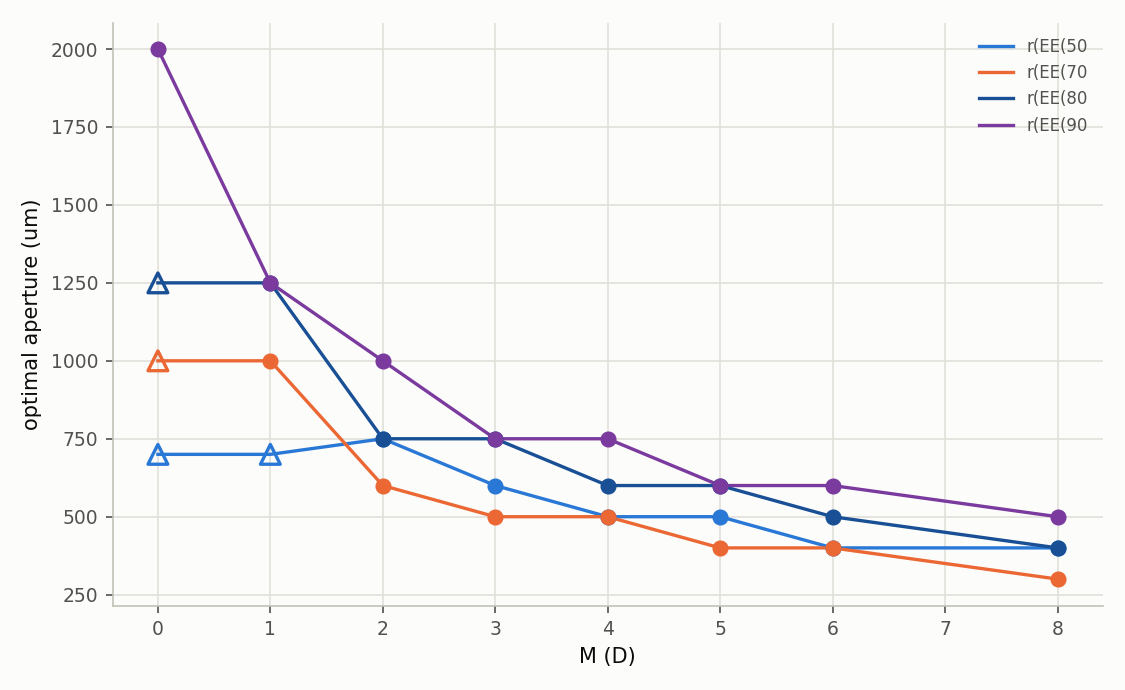
\includegraphics[width=0.85\textwidth]{figures/fig_percentile_optimum_vs_M.png}
\caption{Optimal aperture vs.\ myopia, all four percentiles; hollow markers at $M=0,1$ flag the saturated (non-unique) $r_{EE}(70\%)$/$r_{EE}(80\%)$ points.}
\label{fig:percentile-optimum}
\end{figure}

\section{Reading the genuine ($M\ge2$) rows: $r_{EE}(50\%)$ is systematically biased toward larger apertures}

For every myopia level where the comparison is trustworthy, the optimal aperture by
$r_{EE}(70\%)$ or $r_{EE}(80\%)$ is noticeably \emph{smaller} than by $r_{EE}(50\%)$:
at $M=5\,$D, $500\um$ ($r_{EE}(50\%)$) vs.\ $400\um$ ($r_{EE}(70\%)$); at $M=8\,$D,
$400\um$ vs.\ $300\um$. This is consistent with Chapter~\ref{ch:classical_model}'s
independent finding that $r_{EE}(50\%)$ overestimates real clinical blur by roughly
$7\times$ relative to FWHM: $r_{EE}(50\%)$ stops counting energy before the broader
defocus skirt --- exactly the part of the point-spread function that grows fastest
with aperture at fixed myopia --- starts to matter, so it is systematically biased
toward preferring larger apertures than a percentile that captures more of that skirt.
\textbf{Neither this report nor its source project treats any one percentile as
uniquely correct}; this chapter's purpose is to show, quantitatively, how much the
answer moves depending on which one is chosen, and to flag precisely where that
comparison is (and is not) numerically trustworthy.

\chapter{Deprecated vs.\ Corrected Optics: A Full Comparison}
\label{ch:deprecated_vs_corrected}

Chapter~\ref{ch:physics_audit} presented the before/after optimum-aperture table for a
subset of myopia levels. This chapter re-derives that comparison directly, on the full
$15\times8$ grid, by running the deprecated \texttt{stage2/} pipeline through the
identical sweep machinery used for every corrected-optics result in this report ---
isolated so that it can never contaminate any other chapter's numbers
(Appendix~\ref{app:software}).

\begin{figure}[htbp]
\centering
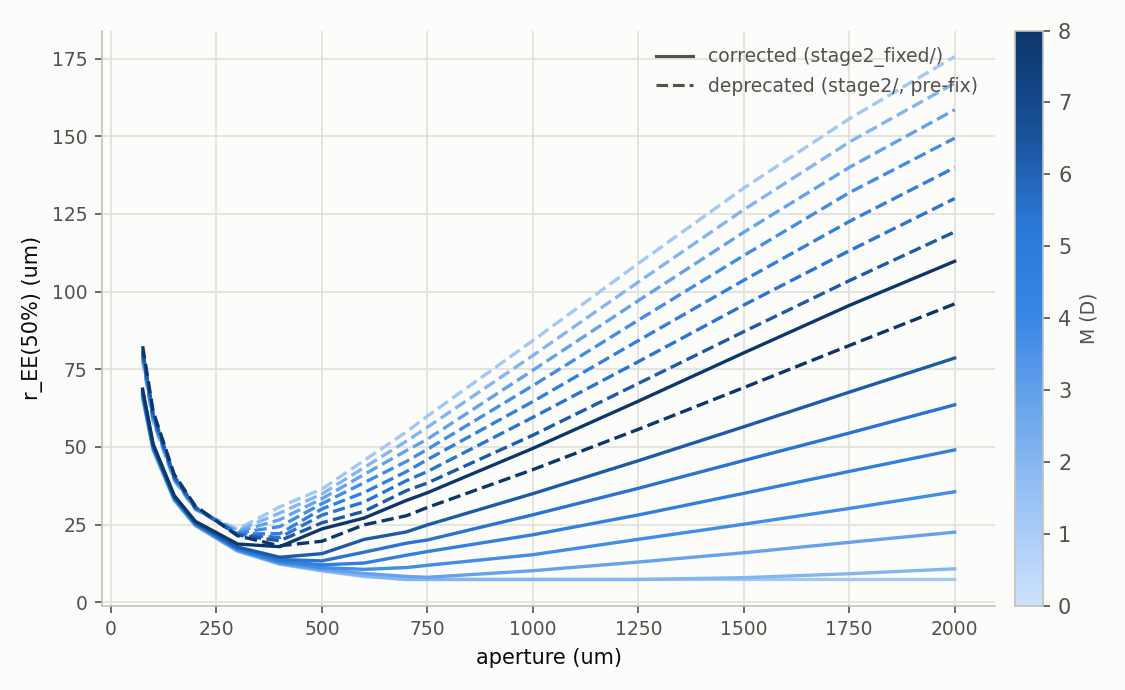
\includegraphics[width=0.85\textwidth]{figures/fig_deprecated_vs_corrected_overlay.png}
\caption{$r_{EE}(50\%)$ vs.\ aperture: corrected optics (solid) vs.\ deprecated pre-fix optics (dashed), one color per myopia level.}
\label{fig:deprecated-vs-corrected}
\end{figure}

{\small
\begin{longtable}{rrrr}
\caption{Optimal aperture, corrected vs. deprecated optics, full grid.}\label{tab:dep-vs-corr-full}\\
\toprule
M (D) & corrected optimum (um) & deprecated optimum (um) & change (\%) \\
\midrule
\endfirsthead
\multicolumn{4}{c}{\tablename\ \thetable\ -- continued}\\
\toprule
M (D) & corrected optimum (um) & deprecated optimum (um) & change (\%) \\
\midrule
\endhead
\bottomrule
\endfoot
0.00 & 700.00 & 300.00 & 133.33 \\
1.00 & 700.00 & 300.00 & 133.33 \\
2.00 & 750.00 & 300.00 & 150.00 \\
3.00 & 600.00 & 300.00 & 100.00 \\
4.00 & 500.00 & 300.00 & 66.67 \\
5.00 & 500.00 & 400.00 & 25.00 \\
6.00 & 400.00 & 400.00 & 0.00 \\
8.00 & 400.00 & 400.00 & 0.00 \\
\end{longtable}
}

The deprecated pipeline reports \emph{uniformly higher} blur radii than the corrected
one at every tested $(a_{hole}, M)$ combination --- consistent with
Chapter~\ref{ch:physics_audit}'s derivation that the bug under-applies the eye lens's
converging power, leaving every point somewhat out of focus relative to where the
corrected pipeline actually places the true focal plane. One further, non-obvious
consequence worth stating plainly: because the deprecated pipeline's blur is uniformly
larger, its retinal spots are less tightly focused, and \textbf{the deprecated pipeline
never exhibits the grid-resolution saturation artifact} of
Chapter~\ref{ch:percentile} at any myopia level tested here --- its own optimum-vs-$M$
table shows no tied minima at all, a coherent, physically sensible side effect of the
bug making every point blurrier rather than an inconsistency in the saturation
diagnosis itself.

\section{Does the fix's impact depend on which percentile is optimized?}

Chapter~\ref{ch:physics_audit}'s headline table used $r_{EE}(50\%)$ only. Repeating
the same corrected-vs-deprecated optimum-aperture comparison at this same spot for
$r_{EE}(70\%)$, $r_{EE}(80\%)$, and $r_{EE}(90\%)$ gives
Figure~\ref{fig:dvc-all-percentiles} and Table~\ref{tab:dvc-all-percentiles}.

\begin{figure}[htbp]
\centering
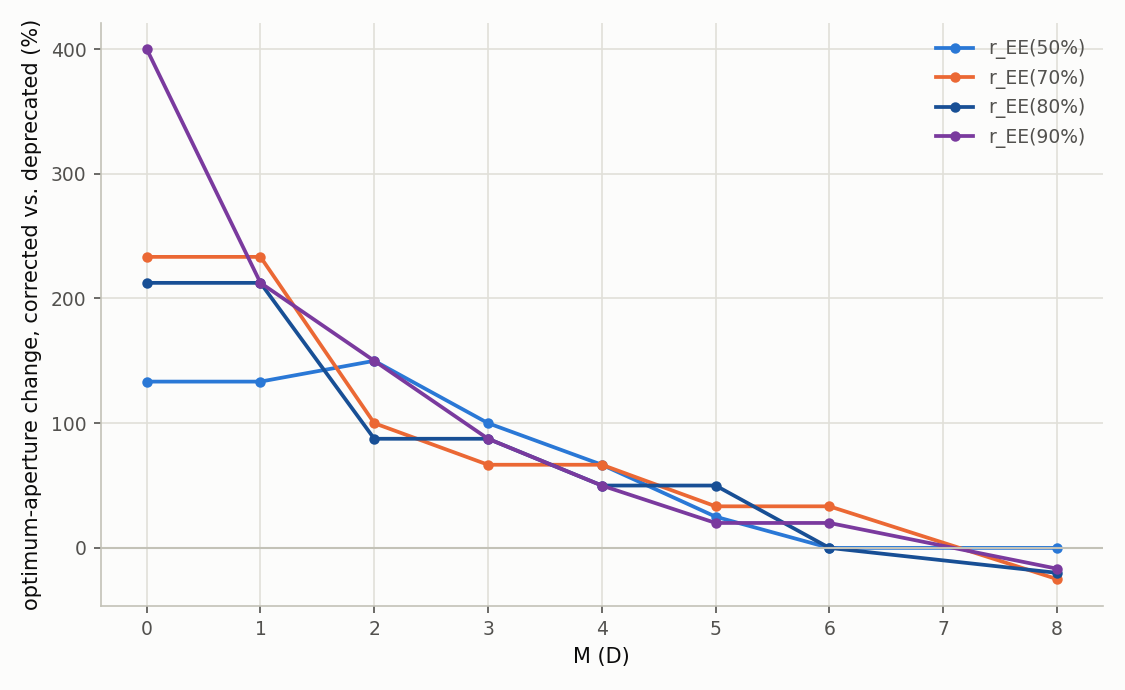
\includegraphics[width=0.85\textwidth]{figures/fig_deprecated_vs_corrected_all_percentiles.png}
\caption{Optimum-aperture change, corrected vs.\ deprecated optics, all four blur percentiles.}
\label{fig:dvc-all-percentiles}
\end{figure}

{\small
\begin{longtable}{rrrrr}
\caption{Optimal-aperture change, corrected vs. deprecated optics (\%), all four percentiles.}\label{tab:dvc-all-percentiles}\\
\toprule
M (D) & r\_EE(50\%) & r\_EE(70\%) & r\_EE(80\%) & r\_EE(90\%) \\
\midrule
\endfirsthead
\multicolumn{5}{c}{\tablename\ \thetable\ -- continued}\\
\toprule
M (D) & r\_EE(50\%) & r\_EE(70\%) & r\_EE(80\%) & r\_EE(90\%) \\
\midrule
\endhead
\bottomrule
\endfoot
0.0 & 133.3 & 233.3 & 212.5 & 400.0 \\
1.0 & 133.3 & 233.3 & 212.5 & 212.5 \\
2.0 & 150.0 & 100.0 & 87.5 & 150.0 \\
3.0 & 100.0 & 66.7 & 87.5 & 87.5 \\
4.0 & 66.7 & 66.7 & 50.0 & 50.0 \\
5.0 & 25.0 & 33.3 & 50.0 & 20.0 \\
6.0 & 0.0 & 33.3 & 0.0 & 20.0 \\
8.0 & 0.0 & -25.0 & -20.0 & -16.7 \\
\end{longtable}
}

The qualitative pattern from Chapter~\ref{ch:physics_audit} --- a large change at low
myopia collapsing toward $0\%$ by $M=6$--$8\,$D --- holds at every percentile, not
only $r_{EE}(50\%)$: the bug's absolute focal-shift error is independent of $M$, so it
dominates the (small) true defocus budget at low $M$ regardless of which blur
percentile measures it, and becomes proportionally negligible at high $M$ for the
same reason across all four. \textbf{Read the $M=0$--$1$ columns for
$r_{EE}(70\%)$/$r_{EE}(80\%)$ with the same caveat as Chapter~\ref{ch:percentile}}:
the corrected-optics side of that percentage change is, at those two myopia levels
specifically, drawn from a saturated (tied, non-unique) optimum, so the exact
percentage shown there is partly an artifact of which tied aperture happened to be
selected, not a fully clean measurement --- the $M\ge2$ columns are unaffected and
trustworthy.

\chapter{Cross-Model Synthesis}
\label{ch:synthesis}

This chapter lays every model's optimal- or representative-aperture answer side by
side. It does not collapse them into one number --- per Chapter~\ref{ch:introduction},
the four objective functions genuinely disagree, and no model in this report clears
the clinical-validation bar (Chapter~\ref{ch:validation}) that would license treating
any one of them as ``the'' answer.

\begin{table}[htbp]
\centering
\small
\begin{tabular}{lll}
\toprule
Source & Aperture range & Basis \\
\midrule
Blur-only optimum, $r_{EE}(50\%)$ (Ch.~\ref{ch:r1sweep}) & $400$--$750\um$ & pure wave-optics blur minimization \\
Blur-only optimum, $r_{EE}(70\%$--$90\%)$ (Ch.~\ref{ch:r1sweep}, \ref{ch:percentile}) & $300$--$1000\um^{\ast}$ & same, alternate percentile ($^\ast$genuine rows only, $M\ge2$D) \\
Brightness-constrained optimum, $M\ge2$D, \emph{any} percentile (Ch.~\ref{ch:stage3a}) & $1000\um$ (exact) & blur-min.\ subject to $6.25\%$ illuminance floor -- percentile-independent once the floor binds \\
Brightness-constrained optimum, $M{=}0$--$1$D (Ch.~\ref{ch:stage3a}) & $1000$--$2000\um$ & percentile-dependent here only, since the floor does not yet bind for $r_{EE}(80\%$--$90\%)$ \\
Deprecated (pre-fix) optimum (Ch.~\ref{ch:deprecated_vs_corrected}) & $300$--$400\um$ & superseded; kept for historical/audit comparison only \\
Clinical bracket (literature/patents) & $940$--$1750\um$ & externally observed range \\
KR 10-2081511 patent & $\sim900\um$ & single stated effective diameter \\
CN 201716487U patent & $400$--$800\um$ & bare geometric assertion, no brightness/ghosting analysis \\
\bottomrule
\end{tabular}
\caption{Every aperture range this report's models or its literature review produced. No single value is endorsed as ``the'' recommendation.}
\label{tab:synthesis}
\end{table}

\section{Reading the pattern across rows}

Two additive corrections move the pure blur-only number toward the observed clinical
range, and their effects are of comparable order: fixing the wavelength bug
(Chapter~\ref{ch:physics_audit}) moved the optimum from $300$--$400\um$ to
$400$--$750\um$ (roughly $\times1.3$ to $\times2.5$, more at low myopia); adding the
brightness floor (Chapter~\ref{ch:stage3a}) moves it further, to exactly $1000\um$ at
every myopia level clinically relevant here ($M\ge2\,$D). Applied together, both
corrections land close to the externally observed clinical bracket's lower-to-middle
region. \textbf{This is a coherent finding, not proof of clinical correctness}: it
shows that two independently-derived, physically-motivated corrections to a naive
blur-only model move the answer in the right direction and roughly the right order of
magnitude --- it is not the same as clinical validation, which Chapter~\ref{ch:validation}
shows this project's own acuity models do not currently achieve.

\textbf{The percentile-choice caveat that runs through Chapters~\ref{ch:r1sweep},
\ref{ch:stage3a}, \ref{ch:percentile}, and~\ref{ch:deprecated_vs_corrected} collapses
to a single, clean statement once the brightness floor is added}: for $M\ge2\,$D, the
brightness-constrained optimum is \emph{exactly} $1000\um$ regardless of which of the
four $r_{EE}(P)$ definitions is used to select it (Section~\ref{sec:stage3a-all-percentiles}).
The percentile-dependence documented at length in Chapter~\ref{ch:percentile} is real
and load-bearing for the \emph{unconstrained} blur-only objective, but is fully
absorbed by the brightness constraint at every myopia level this report treats as
clinically relevant.

\section{What this report does not, and cannot yet, resolve}

\begin{itemize}
\item The $6.25$--$9\%$ brightness floor and the absolute (troland) thresholds
  (Chapter~\ref{ch:brightness_reconciliation}) are not yet reconciled at this
  project's own default scene luminance.
\item No acuity model (closed-form or ideal-observer) predicts either available
  clinical dataset with statistical significance (Chapter~\ref{ch:validation}).
\item Strehl ratio and FWHM are both confirmed unstable in this near-field regime
  (Chapter~\ref{ch:mtf_strehl}) and should not be used as primary design metrics.
\item This entire report is theory-only: \textbf{no physical experiment has been built
  or run} to test any prediction in this document directly.
\end{itemize}

\chapter{Known Limitations}
\label{ch:limitations}

Stated in one place, as an honest list, not a formality --- each item below is
individually documented at the point in this report where it arises; this chapter
exists so a reader never has to reconstruct the full list by re-reading every chapter.

\begin{enumerate}
\item \textbf{Reduced-eye geometry throughout} (Section~\ref{ch:optical_system}): no
  anterior-chamber distance, no cornea/lens power split, single lumped refracting
  plane. Standard, but every pupil/lens-plane distance in this project's pipeline is a
  modeling convenience, not an anatomical one.
\item \textbf{No chromatic aberration, higher-order aberrations, Stiles--Crawford
  apodization in the core PSF, or finite aperture-membrane thickness}
  (Section~\ref{sec:unmodeled}).
\item \textbf{$r_{EE}(P)$ normalizes to grid-captured power, not emitted power}, and is
  measured over a different spatial domain than the threshold-crossing radii
  (Section~\ref{sec:effective-radius}). Both are quantified, not merely flagged, at
  this project's tested configurations.
\item \textbf{$r_{EE}(50\%)$, and at low myopia even $r_{EE}(70\%)$/$r_{EE}(80\%)$, can
  saturate at the simulation grid's own resolution floor}
  (Chapter~\ref{ch:percentile}) --- identified and quantified in this report, not
  previously documented at this level of detail.
\item \textbf{Strehl ratio and FWHM are both confirmed unstable/non-monotonic} in this
  project's near-field operating regime (Chapter~\ref{ch:mtf_strehl}); neither should
  be used as a primary design metric without further work.
\item \textbf{The $6.25$--$9\%$ brightness floor (Chapter~\ref{ch:stage3a}) was
  reverse-engineered to match the known clinical range, not independently derived.}
  A separate absolute-threshold analysis (Chapter~\ref{ch:brightness_reconciliation})
  exists but is not yet fully reconciled against it.
\item \textbf{No acuity predictor --- closed-form or ideal-observer, calibrated or
  uncalibrated --- has passed validation against real clinical data}
  (Chapter~\ref{ch:validation}). This is confirmed, not assumed, and is diagnosed as
  predominantly (though evidence suggests not entirely) a data-scarcity problem: more
  and better public clinical data, not further model tuning, is what this needs.
\item \textbf{The Watson--Yellott pupil--illuminance feedback coupling used throughout
  Stage 4} (Chapter~\ref{ch:stage4}) is a first-principles construction, not itself
  drawn from a single cited source; whether real pupils fully re-equilibrate to it
  within a typical clinical test's timescale is untested.
\item \textbf{This entire report is theory and numerical simulation only.} No physical
  prototype or human-subject experiment has been built or run against any prediction
  in this document.
\end{enumerate}

\section{Suggested priorities for closing these gaps}

Roughly in order of cost vs.\ payoff, per this project's own standing assessment:
(a) reconciling item 6 against item 3's absolute thresholds is the cheapest remaining
task --- both pieces of code already exist and simply need to be run against each
other at a shared, explicitly stated scene-luminance assumption; (b) designing and
running an actual physical/clinical experiment, with per-subject refractive error
recorded (the one fixable flaw every public dataset used in this report shares), would
directly address item 7, the single highest-value open item; (c) further acuity-model
refinement without new data is, per Chapter~\ref{ch:validation}'s own evidence, less
likely to move the outcome than either of the above.

\chapter{Conclusion}

This report has consolidated every single-aperture optimization model this project has
built: an exact wave-optics blur-minimization pipeline, a brightness-constrained
variant of it, a full human-vision acuity layer built on standard photometric and
contrast-sensitivity theory, and a structurally independent ideal-observer Monte Carlo
model built specifically to cross-check the others. It has also consolidated this
project's own audit of itself --- a real, confirmed optical bug, independently
re-derived two ways and fixed, whose correction moved the headline optimum-aperture
number by as much as $150\%$ at some myopia levels; and a separate import-shadowing
bug that meant two of the project's own acuity-validation efforts had, for a period,
never actually tested the pipeline they were built to validate.

The physics is internally consistent and, where checkable against closed-form theory
(the zero-defocus Airy disk, the Fresnel on-axis oscillation formula), matches it
closely. Two independent, physically-motivated corrections --- the wavelength fix and a
brightness-admission floor --- each move the naive blur-only optimum substantially
toward the externally observed clinical bracket, without either fully explaining it
alone. Where this project's models are tested against real clinical acuity data,
however, they do not yet pass: this is reported plainly, with the specific numbers,
rather than reframed as a partial success. The most defensible, load-bearing
conclusion this report can draw is therefore not a single aperture number, but a map
of exactly which models predict what, under which explicit assumptions, and precisely
where each one is --- and is not --- currently validated. Table~\ref{tab:synthesis}
(Chapter~\ref{ch:synthesis}) is that map.

Closing this project's remaining gap between theory and clinical fact, per
Chapter~\ref{ch:limitations}, does not appear to require a fifth acuity model or a
more cleverly parametrized correction term. It requires new, real, per-subject
clinical data, and eventually a physical prototype tested against it --- the one step
this entire body of theoretical work has been building toward and has not yet taken.

\appendix
\chapter{Symbol Table}

\begin{longtable}{@{}lp{7.2cm}l@{}}
\toprule
Symbol & Meaning & Typical value/units \\
\midrule
\endhead
$a_{hole}$ & pinhole diameter & $75$--$2000\um$ \\
$D_{pupil}$ & natural (unobstructed) pupil diameter & $4000\um$ default \\
$d_{gap}$ & pinhole-to-cornea air gap & $12\mm$ default \\
$\lambda$ & vacuum wavelength & $550\,$nm default ($450$/$650\,$nm also used) \\
$\lambda_{eff}$ & effective (vitreous-reduced) wavelength & $\lambda/n'$ \\
$n'$ & vitreous refractive index & $1.336$ \\
$P_0$ & eye's fixed emmetropic power & $60\,$D \\
$M$ & myopia magnitude (excess power) & $0$--$8\,$D \\
$L_0$, $f_{eye}$ & emmetropic axial length / eye focal length & $\approx22.27\mm$ \\
$L_{ax}$, $v_r$ & myopic axial length / retina distance & $n'/(P_0-M)$ \\
$N$, $L$, $dx$ & grid points / window size / pixel pitch & $2048$, $6\mm$, $\approx2.93\um$ \\
$N_F$ & Fresnel number & $(a_{hole}/2)^2/(\lambda z)$ \\
$r_{EE}(P)$ & encircled-energy radius at fraction $P$ & \textmu m \\
$r_{rms}$ & second-moment (RMS) spot radius & \textmu m \\
$S$ & Strehl ratio (this project's own-$M{=}0$-reference convention) & dimensionless \\
$\text{MTF}(f)$, $\text{OTF}(f)$ & modulation/optical transfer function & dimensionless, cycles/degree \\
$\text{CSF}(f)$ & contrast sensitivity function & dimensionless \\
$\text{VSOTF}$ & visual Strehl via OTF (CSF-weighted) & dimensionless \\
$E_{rel}$ & relative retinal illuminance vs.\ full pupil & $[0,1]$ \\
$\text{Td}$ & retinal illuminance, trolands & photopic trolands \\
$\text{MAR}$ & minimum angle of resolution & arcmin \\
$\text{logMAR}$ & $\log_{10}(\text{MAR})$ & dimensionless \\
$T_{min}$ & minimum admissible relative illuminance & $6.25$--$9\%$ \\
$\sigma$ & R7acuity's calibrated neural noise & dimensionless \\
\bottomrule
\end{longtable}

\chapter{Full Data Tables}
\label{app:data}

Every number quoted anywhere in this report comes from one of the CSV files shipped
alongside it (\texttt{new\_sweeps/*.csv} and \texttt{Aperture\_Optimization\_Report/data/*.csv}
--- 11 files, one per sweep, every row machine-checkable). Reproducing all
$120\times3$ raw rows here would add bulk without adding information already
available in those files; this appendix instead gives the complete headline sweep in
full (Table~\ref{tab:app-stage2-blur}, the corrected-optics blur sweep every other
chapter's numbers ultimately derive from) and condensed per-myopia-level summaries of
the other two full-grid sweeps referenced elsewhere in this report.

{\small
\begin{longtable}{rrrrrrr}
\caption{Full Stage 2 (corrected) blur sweep -- all 120 points (the headline dataset this report's Chapter 7 derives from).}\label{tab:app-stage2-blur}\\
\toprule
a\_hole\_um & M\_diopters & r\_EE\_50\_um & r\_EE\_70\_um & r\_EE\_80\_um & r\_EE\_90\_um & rms\_radius\_um \\
\midrule
\endfirsthead
\multicolumn{7}{c}{\tablename\ \thetable\ -- continued}\\
\toprule
a\_hole\_um & M\_diopters & r\_EE\_50\_um & r\_EE\_70\_um & r\_EE\_80\_um & r\_EE\_90\_um & rms\_radius\_um \\
\midrule
\endhead
\bottomrule
\endfoot
75.000 & 0.000 & 65.637 & 89.391 & 110.264 & 233.416 & 259.981 \\
100.000 & 0.000 & 48.858 & 66.390 & 82.571 & 174.659 & 229.338 \\
150.000 & 0.000 & 32.768 & 44.325 & 55.315 & 116.286 & 184.452 \\
200.000 & 0.000 & 24.603 & 33.645 & 41.873 & 87.314 & 160.710 \\
300.000 & 0.000 & 16.403 & 22.210 & 28.168 & 58.225 & 131.041 \\
400.000 & 0.000 & 12.242 & 17.388 & 21.244 & 43.664 & 113.315 \\
500.000 & 0.000 & 10.089 & 13.631 & 18.519 & 35.591 & 101.359 \\
600.000 & 0.000 & 8.252 & 12.256 & 14.258 & 29.084 & 92.487 \\
700.000 & 0.000 & 7.328 & 11.066 & 13.694 & 27.307 & 85.596 \\
750.000 & 0.000 & 7.328 & 10.317 & 13.465 & 25.470 & 82.924 \\
1000.000 & 0.000 & 7.328 & 7.328 & 9.235 & 20.251 & 71.483 \\
1250.000 & 0.000 & 7.328 & 7.328 & 7.328 & 14.018 & 63.653 \\
1500.000 & 0.000 & 7.328 & 7.328 & 7.328 & 13.438 & 57.699 \\
1750.000 & 0.000 & 7.328 & 7.328 & 7.328 & 12.259 & 52.486 \\
2000.000 & 0.000 & 7.328 & 7.328 & 7.328 & 10.499 & 47.590 \\
75.000 & 1.000 & 65.936 & 89.837 & 110.878 & 234.447 & 261.210 \\
100.000 & 1.000 & 49.079 & 66.755 & 83.017 & 175.394 & 230.422 \\
150.000 & 1.000 & 32.928 & 44.578 & 55.586 & 116.739 & 185.325 \\
200.000 & 1.000 & 24.723 & 33.806 & 42.048 & 87.649 & 161.473 \\
300.000 & 1.000 & 16.506 & 22.429 & 28.304 & 58.470 & 131.672 \\
400.000 & 1.000 & 12.334 & 17.588 & 21.411 & 43.894 & 113.875 \\
500.000 & 1.000 & 10.225 & 13.798 & 19.204 & 35.907 & 101.882 \\
600.000 & 1.000 & 8.526 & 12.568 & 14.590 & 30.477 & 92.994 \\
700.000 & 1.000 & 7.328 & 11.734 & 14.355 & 28.236 & 86.103 \\
750.000 & 1.000 & 7.328 & 11.325 & 14.396 & 27.432 & 83.439 \\
1000.000 & 1.000 & 7.328 & 9.243 & 13.608 & 22.824 & 72.076 \\
1250.000 & 1.000 & 7.328 & 10.583 & 13.361 & 20.147 & 64.410 \\
1500.000 & 1.000 & 7.902 & 12.126 & 14.238 & 20.870 & 58.707 \\
1750.000 & 1.000 & 9.161 & 12.791 & 14.606 & 20.968 & 53.857 \\
2000.000 & 1.000 & 10.753 & 13.961 & 17.163 & 21.588 & 49.473 \\
75.000 & 2.000 & 66.279 & 90.293 & 111.494 & 235.720 & 262.481 \\
100.000 & 2.000 & 49.309 & 67.130 & 83.470 & 176.254 & 231.544 \\
150.000 & 2.000 & 33.097 & 44.846 & 55.881 & 117.212 & 186.233 \\
200.000 & 2.000 & 24.858 & 33.993 & 42.268 & 88.114 & 162.272 \\
300.000 & 2.000 & 16.654 & 22.761 & 28.559 & 59.172 & 132.351 \\
400.000 & 2.000 & 12.516 & 18.016 & 21.824 & 45.435 & 114.508 \\
500.000 & 2.000 & 10.564 & 14.241 & 20.915 & 36.628 & 102.514 \\
600.000 & 2.000 & 9.268 & 13.486 & 20.519 & 35.136 & 93.663 \\
700.000 & 2.000 & 8.292 & 13.645 & 19.271 & 31.294 & 86.841 \\
750.000 & 2.000 & 8.011 & 13.972 & 19.079 & 31.067 & 84.222 \\
1000.000 & 2.000 & 10.140 & 15.018 & 20.092 & 28.392 & 73.204 \\
1250.000 & 2.000 & 12.932 & 17.952 & 21.217 & 28.623 & 66.085 \\
1500.000 & 2.000 & 15.919 & 20.734 & 24.563 & 31.034 & 61.141 \\
1750.000 & 2.000 & 19.276 & 24.350 & 27.747 & 34.269 & 57.299 \\
2000.000 & 2.000 & 22.550 & 27.585 & 31.057 & 36.609 & 54.218 \\
75.000 & 3.000 & 66.634 & 90.760 & 112.115 & 236.978 & 263.798 \\
100.000 & 3.000 & 49.548 & 67.514 & 83.932 & 177.294 & 232.708 \\
150.000 & 3.000 & 33.277 & 45.130 & 56.200 & 118.037 & 187.178 \\
200.000 & 3.000 & 25.008 & 34.206 & 42.535 & 88.914 & 163.109 \\
300.000 & 3.000 & 16.848 & 23.209 & 28.939 & 60.322 & 133.080 \\
400.000 & 3.000 & 12.800 & 18.684 & 25.184 & 47.608 & 115.218 \\
500.000 & 3.000 & 11.140 & 16.002 & 24.499 & 42.382 & 103.266 \\
600.000 & 3.000 & 10.571 & 16.364 & 24.230 & 38.688 & 94.507 \\
700.000 & 3.000 & 11.150 & 18.092 & 23.244 & 35.659 & 87.826 \\
750.000 & 3.000 & 11.876 & 18.574 & 22.763 & 34.967 & 85.294 \\
1000.000 & 3.000 & 15.289 & 21.740 & 26.758 & 35.397 & 74.899 \\
1250.000 & 3.000 & 20.253 & 26.202 & 29.945 & 38.568 & 68.703 \\
1500.000 & 3.000 & 25.108 & 30.855 & 35.216 & 42.919 & 64.982 \\
1750.000 & 3.000 & 30.175 & 36.135 & 40.853 & 48.180 & 62.671 \\
2000.000 & 3.000 & 35.546 & 41.966 & 46.169 & 53.084 & 61.427 \\
75.000 & 4.000 & 67.001 & 91.238 & 112.740 & 238.218 & 265.163 \\
100.000 & 4.000 & 49.796 & 67.910 & 84.403 & 178.311 & 233.915 \\
150.000 & 4.000 & 33.467 & 45.429 & 56.544 & 118.872 & 188.161 \\
200.000 & 4.000 & 25.176 & 34.448 & 42.849 & 89.727 & 163.986 \\
300.000 & 4.000 & 17.095 & 23.778 & 29.983 & 61.582 & 133.864 \\
400.000 & 4.000 & 13.203 & 19.611 & 29.211 & 49.930 & 116.012 \\
500.000 & 4.000 & 12.016 & 19.519 & 28.091 & 45.790 & 104.145 \\
600.000 & 4.000 & 12.603 & 21.432 & 27.055 & 41.806 & 95.540 \\
700.000 & 4.000 & 15.117 & 21.662 & 27.977 & 41.116 & 89.076 \\
750.000 & 4.000 & 16.301 & 21.971 & 28.890 & 40.943 & 86.675 \\
1000.000 & 4.000 & 21.706 & 28.413 & 33.707 & 43.389 & 77.181 \\
1250.000 & 4.000 & 28.086 & 34.898 & 39.953 & 48.787 & 72.261 \\
1500.000 & 4.000 & 35.038 & 42.067 & 47.008 & 55.708 & 70.143 \\
1750.000 & 4.000 & 42.099 & 49.234 & 54.183 & 62.814 & 69.723 \\
2000.000 & 4.000 & 49.028 & 57.007 & 62.190 & 70.385 & 70.602 \\
75.000 & 5.000 & 67.380 & 91.729 & 113.370 & 239.446 & 266.579 \\
100.000 & 5.000 & 50.054 & 68.317 & 84.884 & 179.312 & 235.168 \\
150.000 & 5.000 & 33.670 & 45.746 & 56.913 & 119.698 & 189.186 \\
200.000 & 5.000 & 25.361 & 34.721 & 43.211 & 90.552 & 164.906 \\
300.000 & 5.000 & 17.400 & 24.470 & 32.774 & 62.917 & 134.706 \\
400.000 & 5.000 & 13.749 & 20.820 & 32.735 & 53.542 & 116.896 \\
500.000 & 5.000 & 13.289 & 23.363 & 30.950 & 48.586 & 105.163 \\
600.000 & 5.000 & 16.108 & 24.949 & 29.943 & 45.486 & 96.774 \\
700.000 & 5.000 & 18.985 & 26.766 & 33.241 & 46.424 & 90.608 \\
750.000 & 5.000 & 20.028 & 28.185 & 34.200 & 47.145 & 88.382 \\
1000.000 & 5.000 & 28.134 & 35.496 & 41.319 & 51.965 & 80.064 \\
1250.000 & 5.000 & 36.663 & 43.912 & 49.530 & 59.311 & 76.729 \\
1500.000 & 5.000 & 45.603 & 53.538 & 58.883 & 68.534 & 76.503 \\
1750.000 & 5.000 & 54.448 & 63.255 & 68.833 & 78.045 & 78.198 \\
2000.000 & 5.000 & 63.545 & 72.970 & 78.808 & 87.602 & 81.324 \\
75.000 & 6.000 & 67.773 & 92.233 & 114.006 & 240.668 & 268.048 \\
100.000 & 6.000 & 50.323 & 68.736 & 85.375 & 180.300 & 236.470 \\
150.000 & 6.000 & 33.885 & 46.080 & 57.309 & 120.518 & 190.254 \\
200.000 & 6.000 & 25.566 & 35.027 & 43.624 & 91.391 & 165.872 \\
300.000 & 6.000 & 17.769 & 25.292 & 35.574 & 64.298 & 135.612 \\
400.000 & 6.000 & 14.472 & 23.107 & 35.635 & 58.689 & 117.877 \\
500.000 & 6.000 & 15.631 & 26.864 & 33.719 & 51.256 & 106.329 \\
600.000 & 6.000 & 20.210 & 27.956 & 36.183 & 50.925 & 98.225 \\
700.000 & 6.000 & 22.620 & 31.909 & 38.139 & 51.051 & 92.438 \\
750.000 & 6.000 & 24.880 & 33.517 & 39.991 & 52.472 & 90.433 \\
1000.000 & 6.000 & 34.940 & 43.017 & 49.402 & 60.936 & 83.551 \\
1250.000 & 6.000 & 45.543 & 54.025 & 60.094 & 70.924 & 82.065 \\
1500.000 & 6.000 & 56.467 & 65.480 & 71.793 & 81.810 & 83.940 \\
1750.000 & 6.000 & 67.609 & 77.726 & 84.031 & 93.946 & 87.877 \\
2000.000 & 6.000 & 78.595 & 89.999 & 96.234 & 106.191 & 93.298 \\
75.000 & 8.000 & 68.599 & 93.282 & 115.299 & 243.523 & 271.159 \\
100.000 & 8.000 & 50.897 & 69.614 & 86.389 & 182.262 & 239.230 \\
150.000 & 8.000 & 34.357 & 46.805 & 58.182 & 122.158 & 192.532 \\
200.000 & 8.000 & 26.042 & 35.745 & 45.715 & 93.110 & 167.953 \\
300.000 & 8.000 & 18.737 & 27.356 & 44.014 & 72.213 & 137.631 \\
400.000 & 8.000 & 17.874 & 31.333 & 40.205 & 63.135 & 120.163 \\
500.000 & 8.000 & 23.600 & 32.951 & 41.933 & 58.812 & 109.149 \\
600.000 & 8.000 & 27.088 & 37.986 & 44.609 & 61.606 & 101.829 \\
700.000 & 8.000 & 32.756 & 42.622 & 49.662 & 64.499 & 97.056 \\
750.000 & 8.000 & 35.242 & 45.157 & 52.101 & 66.674 & 95.626 \\
1000.000 & 8.000 & 49.513 & 59.879 & 66.507 & 79.844 & 92.333 \\
1250.000 & 8.000 & 64.708 & 75.585 & 82.727 & 94.800 & 95.149 \\
1500.000 & 8.000 & 80.262 & 92.060 & 99.265 & 110.862 & 101.624 \\
1750.000 & 8.000 & 95.523 & 108.631 & 116.075 & 127.857 & 110.245 \\
2000.000 & 8.000 & 109.754 & 125.697 & 133.430 & 145.104 & 120.312 \\
\end{longtable}
}
{\small
\begin{longtable}{rrrrr}
\caption{Stage 4 acuity sweep, condensed per myopia level (full 120-point grid in new\_sweeps/acuity\_sweep\_stage4.csv).}\label{tab:app-stage4}\\
\toprule
M (D) & best aperture (um) & min logMAR & max logMAR & mean logMAR \\
\midrule
\endfirsthead
\multicolumn{5}{c}{\tablename\ \thetable\ -- continued}\\
\toprule
M (D) & best aperture (um) & min logMAR & max logMAR & mean logMAR \\
\midrule
\endhead
\bottomrule
\endfoot
0.000 & 2000.000 & -0.344 & 1.121 & 0.255 \\
1.000 & 1250.000 & -0.120 & 1.116 & 0.356 \\
2.000 & 750.000 & 0.076 & 1.111 & 0.482 \\
3.000 & 750.000 & 0.112 & 1.106 & 0.564 \\
4.000 & 600.000 & 0.181 & 1.101 & 0.641 \\
5.000 & 600.000 & 0.240 & 1.123 & 0.705 \\
6.000 & 500.000 & 0.259 & 1.203 & 0.765 \\
8.000 & 400.000 & 0.331 & 1.330 & 0.859 \\
\end{longtable}
}
{\small
\begin{longtable}{rrrrr}
\caption{Deprecated (pre-fix) Stage 2 blur sweep, condensed per myopia level (full 120-point grid in Aperture\_Optimization\_Report/data/stage2\_deprecated\_sweep.csv).}\label{tab:app-stage2-dep}\\
\toprule
M (D) & best aperture (um) & min r\_EE50 (um) & max r\_EE50 (um) & mean r\_EE50 (um) \\
\midrule
\endfirsthead
\multicolumn{5}{c}{\tablename\ \thetable\ -- continued}\\
\toprule
M (D) & best aperture (um) & min r\_EE50 (um) & max r\_EE50 (um) & mean r\_EE50 (um) \\
\midrule
\endhead
\bottomrule
\endfoot
0.000 & 300.000 & 23.487 & 175.621 & 74.230 \\
1.000 & 300.000 & 23.044 & 167.080 & 71.203 \\
2.000 & 300.000 & 22.645 & 158.517 & 68.090 \\
3.000 & 300.000 & 22.293 & 149.369 & 64.870 \\
4.000 & 300.000 & 21.987 & 139.909 & 61.465 \\
5.000 & 400.000 & 20.830 & 129.938 & 58.058 \\
6.000 & 400.000 & 19.792 & 119.210 & 54.475 \\
8.000 & 400.000 & 18.158 & 96.032 & 46.952 \\
\end{longtable}
}

\chapter{Software Architecture Note}
\label{app:software}

\section{Provenance of every number in this report}

Every sweep in this report was produced by directly calling this project's own
pre-existing, independently-tested compute functions --- never a re-derivation written
specifically for this document. Concretely, every figure and table traces to one of:
(a) \texttt{new\_sweeps/blur\_sweep.csv} and \texttt{acuity\_sweep\_stage4.csv}, this
project's own most recent full-grid corrected-optics runs (Chapters~\ref{ch:r1sweep}
and~\ref{ch:stage4}); or (b) a fresh run of \texttt{master\_dashboard/wrappers.py}'s
thin wrapper functions, generated specifically for this report by this report's own
\texttt{generate\_report\_data.py} --- the same functions that back this project's
live interactive dashboard, so every number here is independently reproducible by
running that dashboard.

\section{The deprecated-optics isolation mechanism}

Chapter~\ref{ch:deprecated_vs_corrected}'s comparison requires deliberately loading
the pre-fix \texttt{stage2/} optics module --- the one piece of this report's pipeline
that must, by design, differ from every other chapter's \texttt{stage2\_fixed/}-based
result. \texttt{stage2/} and \texttt{stage2\_fixed/} define same-named Python modules
(\texttt{phase2\_retina}, \texttt{myopia\_axial}, \texttt{pipeline\_junction}); since
Python caches imports by bare module name process-wide, a naive import of the
deprecated copy risks \emph{permanently shadowing} the corrected copy for every other
chapter's sweep run afterward in the same process --- precisely the failure mode
documented in Chapter~\ref{ch:validation}.

This is avoided with an isolated import context manager
(\texttt{wrappers.\_isolated\_\allowbreak stage2\_deprecated\_\allowbreak import()}) that: (1) saves whatever is
currently cached under the three colliding names; (2) removes \texttt{stage2\_fixed/}
from the Python import path and inserts \texttt{stage2/} in its place, for the
duration of one sweep call only; (3) asserts the freshly-imported module resolves to
the expected deprecated file path, refusing to proceed otherwise; (4) on exit,
restores the original path and cached modules, and \textbf{re-verifies} that the
corrected pipeline is exactly as it was before --- raising a fatal error, not a silent
pass-through, if it is not. This was independently tested, not merely asserted to
work: a corrected-optics sweep run immediately before and immediately after the
deprecated-optics sweep in Chapter~\ref{ch:deprecated_vs_corrected} produces
bit-for-bit identical results.

\section{Registry-driven dashboard architecture}

\texttt{master\_dashboard/} --- the live, interactive companion to this static report
--- is built on one design principle relevant to how this report's own data was
produced: every stage is one entry in a single registry dict
(\texttt{master\_dashboard/registry.py}) mapping a stage key to its real entry point,
parameter widgets, and output shape; the dashboard's own UI code contains no
stage-specific physics, sweep loops, or plotting math anywhere. This report's data
generator (\S B.1 above) calls the identical wrapper functions that registry points
at, so this report and the live dashboard are guaranteed to agree, not two
independently-maintained sources of the same numbers.


\end{document}
